\documentclass{beamer}

\mode<presentation>
{
	\usepackage{StyleFiles/Rome}
	\setbeamercovered{transparent}
}

\mode<handout>
{
	\usepackage{pgfpages}
	\pgfpagesuselayout{2 on 1}[a4paper,border shrink=5mm]
	\nofiles
}

\usepackage[english]{babel}
\usepackage[algoruled]{algorithm2e}
\usepackage{movie15}
\usepackage{rotating}
\usepackage{subfigure}

\definecolor{darkgreen}{RGB}{0,180,0}
\definecolor{lightred}{RGB}{210,0,0}

\setbeamertemplate{itemize subitem}{\tiny\raise1.5pt\hbox{\donotcoloroutermaths$ \blacktriangleright $}}

\title[Predicting Future Agent Motions through a Distributed Multi-Clustered PF]{\Large Predicting Future Agent Motions through a Distributed Multi- Clustered Particle Filtering}

\subtitle{}

\author[Fabio Previtali]{\Large\textbf{Fabio Previtali}}

\date[May 9, 2016]{Learning in Autonomous Systems\\A.Y. 2015/2016\\Rome, Italy}

\begin{document}

\begin{frame}[plain]
	\titlepage
\end{frame}

\section{Introduction}

\begin{frame}
	\frametitle{Challenging Problem}
	
	\begin{center}
		\begin{tikzpicture}
			\node at (0,0) [draw=white,ultra thick,inner sep=0pt]
			{
				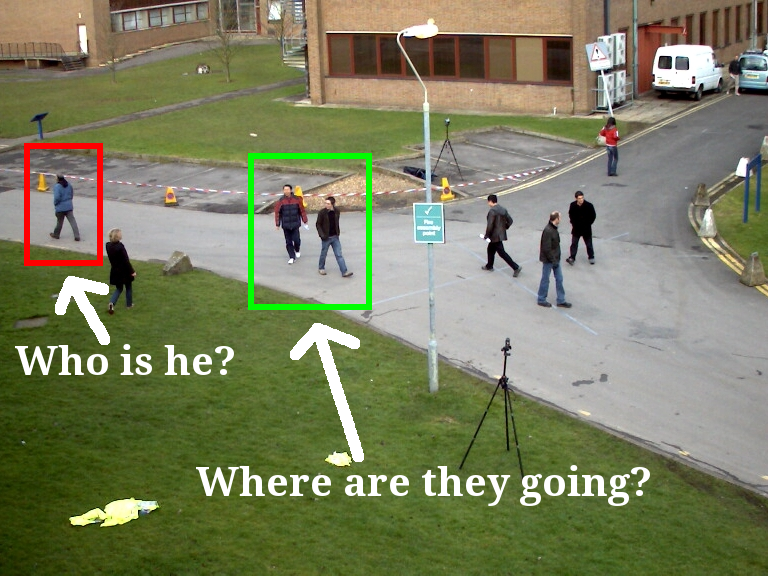
\includegraphics[width=\linewidth]{Figures/Problem.png}
			};
		\end{tikzpicture}
	\end{center}
\end{frame}

\begin{frame}
	\frametitle{Motivation}
	
	\vspace{0.2cm}
	
	\Large
	
	\begin{block}{Objective}
		\textbf{Understanding} the concept of human preference \textbf{allows} to perform higher levels
		of reasoning about future human actions. Likewise, the \textbf{knowledge} of a goal also gives
		information about \textbf{what} a person might do
	\end{block}
	
	\vspace{0.3cm}
	
	Example of application fields:
	\begin{itemize}
		\item Automatic video surveillance
		\item Human-Robot Interaction
		\item Domestic robots
	\end{itemize}
\end{frame}

\begin{frame}
	\frametitle{Contributions}
	
	\Large
	
	The main contributions of this thesis are:
	
	\begin{enumerate}
		\item \textbf{Distributed real-time} multiple object tracking
		\item \textbf{Asynchronous} and \textbf{fully} scalable design
		\item \textbf{Prediction} without prior scene semantics knowledge
		\item \textbf{Incremental} updates of the \emph{IRL} model over time
		\item \textbf{Non-uniform grids} for representing world state
		\item \textbf{Efficient} and \textbf{scalable} solution for on-robot implementation
	\end{enumerate}
\end{frame}

\begin{frame}
	\frametitle{Proposed Solution}
	
	\vspace{0.5cm}
	
	\begin{tikzpicture}
		\node at (0,0) [draw=white,ultra thick,inner sep=0pt]
		{
			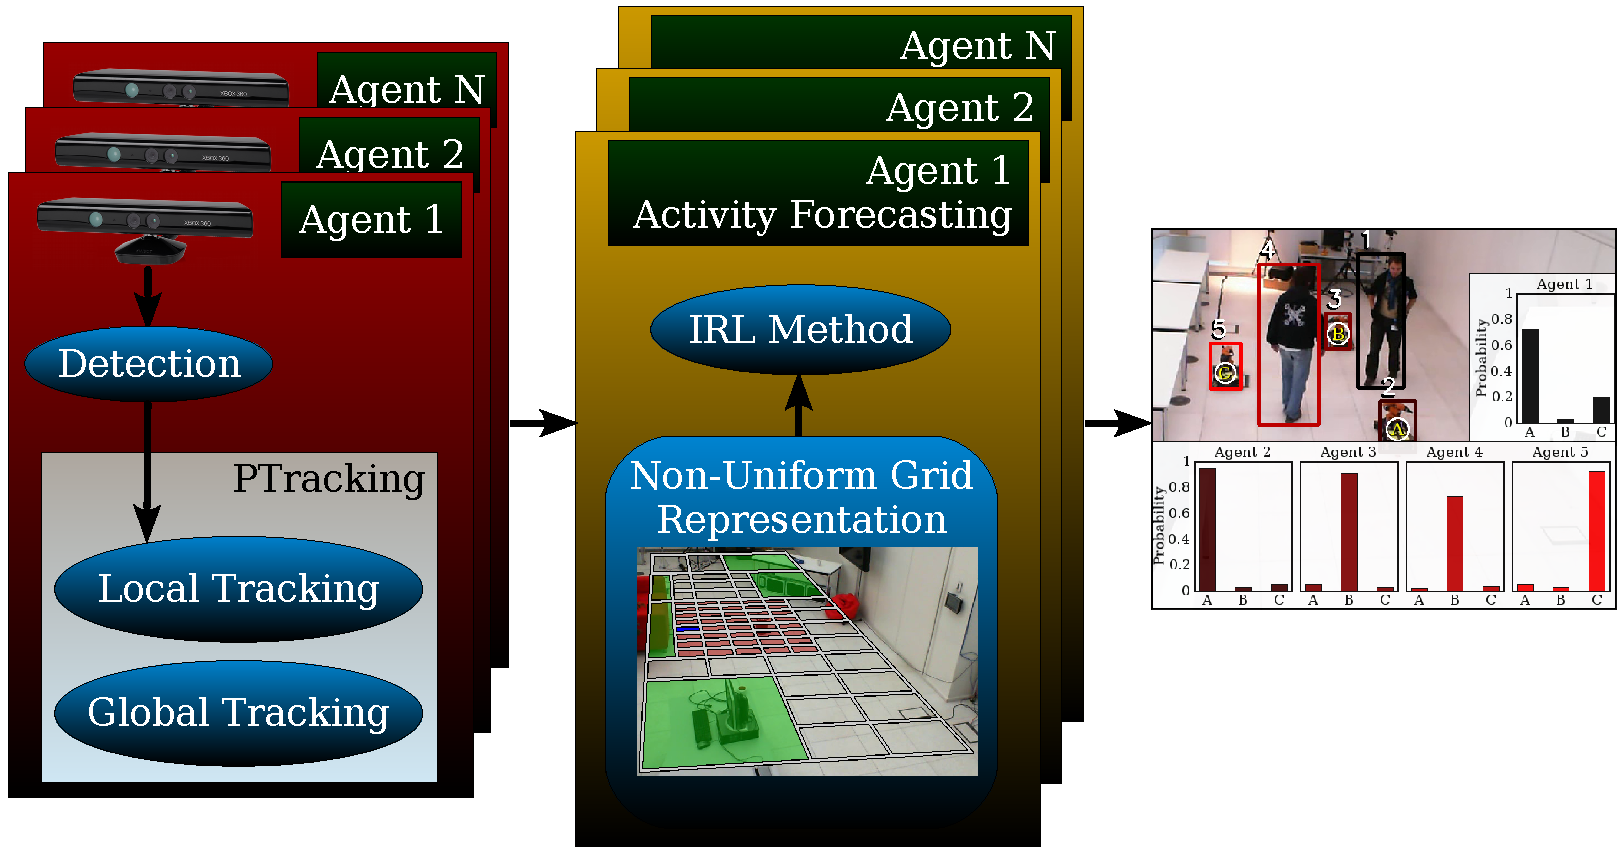
\includegraphics[width=\linewidth]{Figures/Architecture}
		};
	\end{tikzpicture}
\end{frame}

\section{Handson}

\begin{frame}
	\frametitle{Hands-on PTracking}
	\framesubtitle{Getting the library}
	
	\emph{PTracking} is currently available in the following private GitHub repository:
	\begin{center}
		\url{https://github.com/fabioprev/ptracking}
	\end{center}
	
	A request for getting access is required:
	\begin{center}
		\url{previtali@dis.uniroma1.it}
	\end{center}
	
	Currently the only supported development platform is \textbf{Linux}.
\end{frame}

\begin{frame}
	\frametitle{Hands-on PTracking}
	\framesubtitle{Dependencies}
	
	On Xubuntu (Ubuntu) 14.04 LTS (kernel 3.13.0-37) and later versions, you need to install
	the following packages
	
	\vspace{0.2cm}
	
	\begin{columns}[T]
		\column{.5\textwidth}
		
		\begin{itemize}
			\item build-essential
			\item cmake
			\item libxml2
			\item libxml2-dev
			\item libboost1.54-all-dev
		\end{itemize}
		
		\column{.5\textwidth}
		\centering
		
		\begin{itemize}
			\item libcgal-dev
			\item libopencv-dev
			\item libopenni2-dev (optional)
			\item gnuplot (optional)
			\item gnuplot-x11 (optional)
		\end{itemize}
	\end{columns}
\end{frame}

\begin{frame}
	\frametitle{Hands-on PTracking}
	\framesubtitle{Building the library}
	
	We recommend a so-called out of source build which can be achieved by the following command
	sequence
	
	\vspace{0.2cm}
	
	\begin{itemize}
		\item \texttt{cd <PTracking-root-directory>}
		\item \texttt{mkdir build}
		\item \texttt{cd build}
		\item \texttt{cmake ../src}
		\item \texttt{make -j<number-of-cores+1>}
	\end{itemize}
\end{frame}

\begin{frame}
	\frametitle{Hands-on PTracking}
	\framesubtitle{Installing the library}
	
	\vspace{0.4cm}
	
	The library can be optionally installed by typing the following command sequence
	
	\vspace{0.2cm}
	
	\begin{itemize}
		\item \texttt{cd <PTracking-root-directory>/build}
		\item \texttt{sudo make install}
	\end{itemize}
	
	\vspace{0.15cm}
	
	\textbf{Header files:} \texttt{/usr/local/include/PTracking} \\
	
	\vspace{0.15cm}
	
	\textbf{Shared objects:} \texttt{/usr/local/lib/PTracking} \\
	
	\vspace{0.15cm}
	
	\textbf{Binaries:} \texttt{/usr/local/bin} \\
	
	\vspace{0.75cm}
	
	\textbf{Warning:} You first need to logout before starting using the library, because the
	\texttt{$ \sim $/.profile} file has been modified
\end{frame}

\begin{frame}
	\frametitle{Project}
	
	\vspace{0.5cm}
	
	\setstretch{1}
	To whom is interested in doing a project about multiple object tracking using heterogeneous
	sensors, just need to drop me an email at \url{previtali@dis.uniroma1.it}\\
	
	\vspace{-0.3cm}
	
	\begin{center}
		\begin{tikzpicture}
			\node at (0,0) [draw=white,ultra thick,inner sep=0pt]
			{
				\includegraphics[scale=0.23]{Figures/IRL-Model.png}
			};
		\end{tikzpicture}
	\end{center}
\end{frame}

\section{Related Work}

\begin{frame}
	\frametitle{Related Work}
	\framesubtitle{Multi-object tracking}
	
	\Large
	
	\vspace{0.4cm}
	
	Multi-object tracking algorithms can be classified into two groups (Andriyenko \emph{et al.}):
	
	\vspace{0.2cm}
	
	\begin{itemize}
		\item \textbf{Global} (or \emph{offline}): formulating the tracking problem as an
			  optimization one, where all the trajectories within a temporal window are
			  optimized jointly
		\item \textbf{Recursive} (or \emph{online}): estimating the current state relying
			  only on the current observations and on the previous state
	\end{itemize}
\end{frame}

%\begin{frame}
%	\frametitle{Multi-Object Tracking}
%	\framesubtitle{Global methods}
%	
%	\Large
%	
%	\vspace{0.2cm}
%	
%	\begin{itemize}
%		\item \textbf{Berclaz} \emph{et al.} \cite{Berclaz11}: mathematically sound
%			  multiple object tracking framework based on a k-shortest path optimization
%			  algorithm
%		\vspace{0.1cm}
%		\item \textbf{Leal-Taix{\'e}} \emph{et al.} \cite{Leal11}: formulate a new graph
%			  model for the multiple object tracking challenge by minimizing a network flow
%			  problem
%		\vspace{0.1cm}
%		\item \textbf{Sharma} \emph{et al.} \cite{Sharma09}: adapting a Cluster-Boosted
%			  Tree based pedestrian detector to deal with the people tracking problem
%		\vspace{0.1cm}
%		\item ...
%	\end{itemize}
%\end{frame}
%
%\begin{frame}
%	\frametitle{Multi-Object Tracking}
%	\framesubtitle{Recursive methods}
%	
%	\Large
%	
%	\vspace{0.2cm}
%	
%	\begin{itemize}
%		\item \textbf{Breitenstein} \emph{et al.} \cite{Breitenstein11}: online method for
%			  multi-person tracking-by-detection in a particle filtering framework
%		\vspace{0.1cm}
%		\item \textbf{Yang} \emph{et al.} \cite{Yang09}: probabilistic appearance model
%			  method for tracking multiple people
%		\vspace{0.1cm}
%		\item ...
%	\end{itemize}
%\end{frame}

\begin{frame}
	\frametitle{Global vs Recursive Methods}
	
	\begin{table}[!t]
		\centering
		\begin{tabular}{ c | c | c | }
			\cline{2-3}
			& \textbf{Global Methods} & \textbf{Recursive Methods} \\ \hline
			
			\multicolumn{1}{|c|}{\textbf{Accuracy}} & medium/high & medium/high \\ \hline
			\multicolumn{1}{|c|}{\textbf{Precision}} & \textbf{high} & medium/high \\ \hline
			\multicolumn{1}{|c|}{\textbf{Robustness}} & \textbf{high} & medium/high \\ \hline
			\multicolumn{1}{|c|}{\textbf{Computational Load}} & high & \textbf{low}/medium \\ \hline
			\multicolumn{1}{|c|}{\textbf{Real-time}} & no & \textbf{yes}/no \\ \hline
		\end{tabular}
	\end{table}
	
	\vspace{0.4cm}
	
	Global methods are more precise and more robust but, on the other hand, they
	cannot run in a real system because:
	
	\begin{itemize}
		\item no information from the future are available (offline computation)
		\item frame rate not suitable for real-time applications
	\end{itemize}
\end{frame}

\section{PTracking Algorithm}

\begin{frame}
	\frametitle{}
	
	\Huge
	
	\vspace{0.5cm}
	
	\begin{center}
		\textbf{PTracking}
	\end{center}
\end{frame}

\begin{frame}
	\frametitle{PTracking}
	\framesubtitle{Distributed Particle Filtering for Multi-Sensor Multiple Object Tracking}
	
	\LARGE
	
	\begin{block}{Idea}
		Achieving \textbf{high} precision and robustness, as a global method does, while trying to keep
		a \textbf{low} computational load in order to obtain \textbf{real-time} performance, as
		recursive methods do
	\end{block}
\end{frame}

\begin{frame}
	\frametitle{PTracking}
	\framesubtitle{Contributions}
	
	\Large
	
	\vspace{0.2cm}
	
	We propose a novel technique based on \emph{Distributed Particle Filtering}. The key contributions
	are:
	
	\vspace{0.15cm}
	
	\begin{enumerate}
		\item \textbf{Real-time} multiple object tracking method
		\item Novel clustering method that \textbf{keeps} track of multiple objects whose number is
			  \textbf{not known} a priori, ensuring a \textbf{limited} Gaussian distribution in the
			  particle space
		\item \textbf{Asynchronous} algorithm to improve robustness with respect to communication
			  failures and dead nodes
	\end{enumerate}
\end{frame}

\begin{frame}
	\frametitle{PTracking}
	\framesubtitle{General Schema}
	
	\vspace{-0.27cm}
	
	\begin{columns}[T]
		\column{.5\textwidth}
		
		\vspace{0.8cm}
		
		\begin{itemize}
			\item \textbf{Input:} set of positions of the objects provided by a multi object detector
				  system (e.g., \cite{Bloisi12})
			
			\vspace{1.6cm}
			
			\item \textbf{Output:} set of estimated trajectories of the moving objects over time
		\end{itemize}
		
		\column{.5\textwidth}
		\centering
		
		\begin{tikzpicture}
			\node at (0,0) [draw=black,ultra thick,inner sep=0pt]
			{
				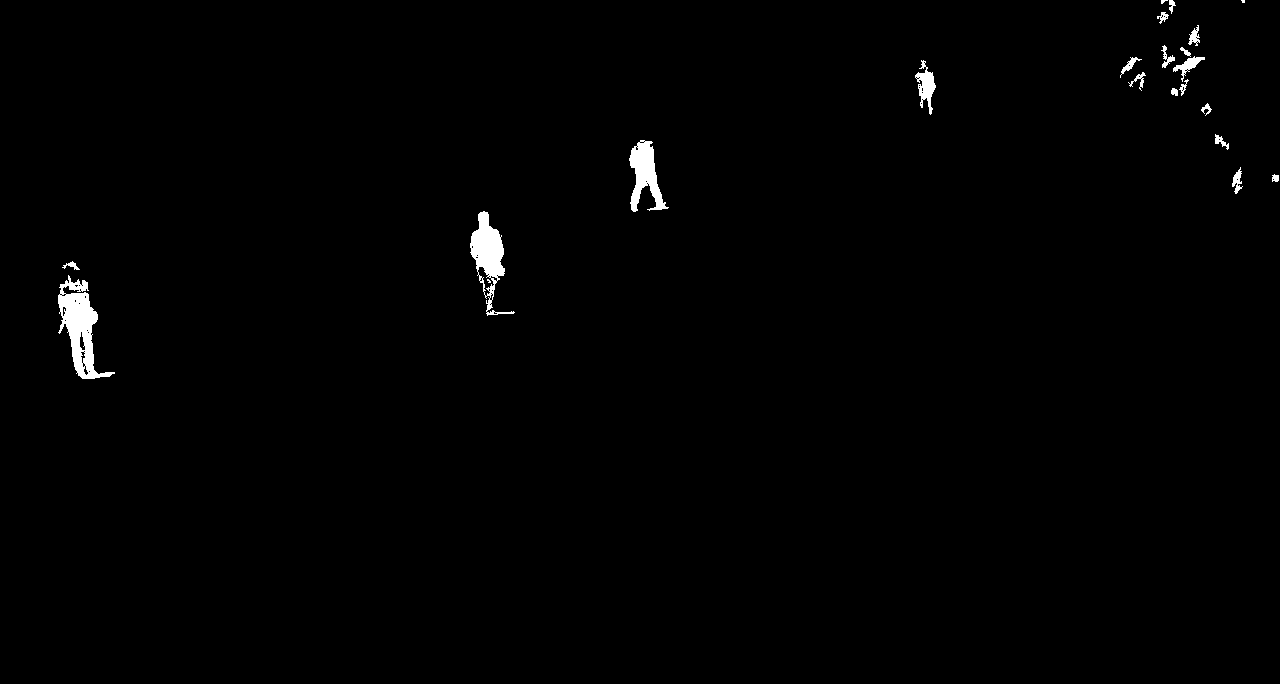
\includegraphics[width=6cm]{Figures/Detection}
			};
			\node at (0,-3.35) [draw=black,ultra thick,inner sep=0pt]
			{
				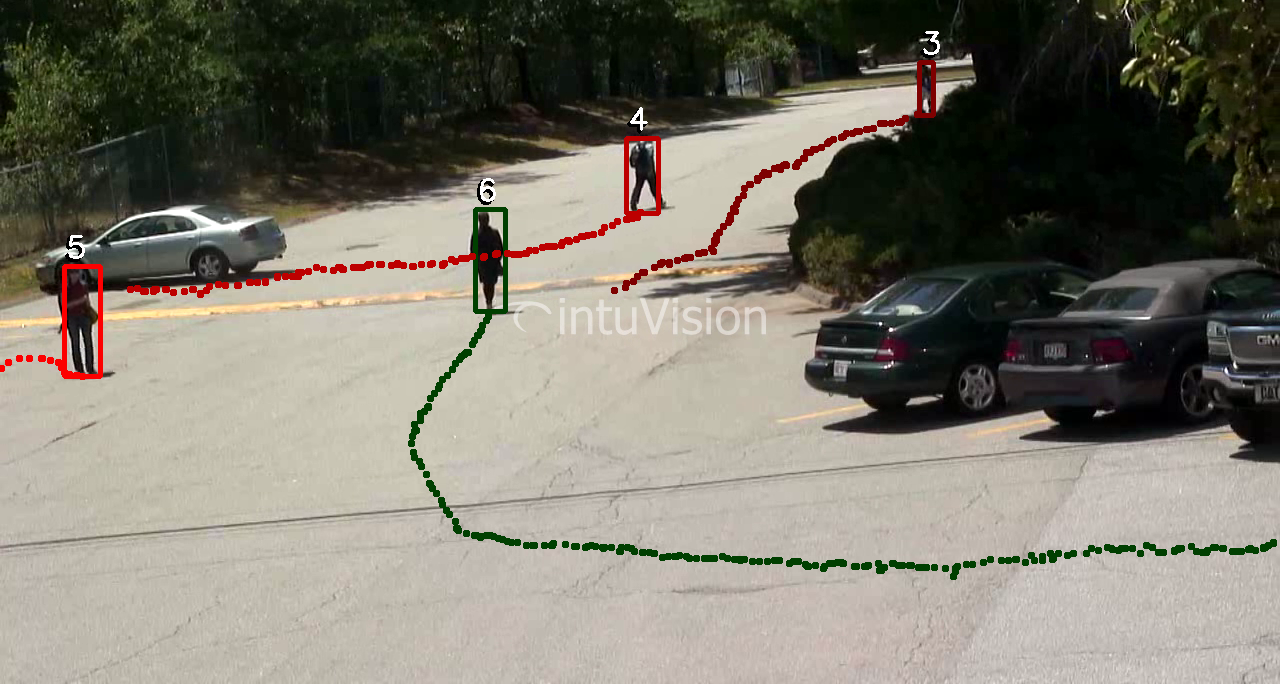
\includegraphics[width=6cm]{Figures/Tracking}
			};
		\end{tikzpicture}
	\end{columns}
	
	\vspace{0.3cm}
	
	\tiny
	
	\cite{Bloisi12} D. D. Bloisi \emph{et al.},  ``Independent Multimodal Background Subtraction'',
	CompIMAGE, 2012
\end{frame}

\begin{frame}
	\frametitle{PTracking}
	\framesubtitle{Pseudo-code}
	
	\begin{columns}[T]
		\column{.05\textwidth}
		
		\column{.55\textwidth}
		
		\only<1>
		{
			\begin{algorithm}[H]
				\tiny
				\KwIn{perceptions $ z_{s,t} $, local track numbers $ oi_{s,t-1} $, global track numbers $ OI_{s,t-1} $}
				\BlankLine
				\KwData{set of local particles $ \tilde{\xi}_{s,t} $, set of global particles $ \tilde{\xi}_{\mathcal{S'},t} $, sensor pose $ m_{s,t} $, local GMM set $ \mathcal{L} $, global GMM set $ \mathcal{G} $}
				\BlankLine
				\KwOut{global estimations $ x_{s,t} = (\boldsymbol{OI}_{s,t},\boldsymbol\Lambda_{s,t},\boldsymbol{M}_{s,t},\boldsymbol\Sigma_{s,t}) $}
				\BlankLine
				\Begin
				{
					\textcolor{darkgreen}{$ \tilde{\xi}_{s,t} \sim \pi_t (x_{s,t} | x_{s,t-1},z_{s,t},m_{s,t}) $}
					\BlankLine
					\textcolor{darkgreen}{Re-sample by using the SIR principle}\\
					\BlankLine
					\textcolor{darkgreen}{$ \mathcal{L} = KClusterize(\tilde{\xi}_{s,t}) $}
					\BlankLine
					\textcolor{darkgreen}{$ (\boldsymbol{oi}_{s,t},\boldsymbol\lambda_{s,t},\boldsymbol\mu_{s,t},\boldsymbol\sigma_{s,t}) = DataAssociation(\mathcal{L}, oi_{s,t-1}) $}
					\BlankLine
					\textcolor{darkgreen}{Communicate belief $ (\boldsymbol{oi}_{s,t},\boldsymbol\lambda_{s,t},\boldsymbol\mu_{s,t},\boldsymbol\sigma_{s,t}) $ to other agents}
				}
				\BlankLine
				\Begin
				{
					Collect $ \mathcal{L}_{S'} $ from a subset $ \mathcal{S'} \subseteq \mathcal{S} $ of
					sensors within a $ \Delta t $
					\BlankLine
					$ \tilde{\xi}_{\mathcal{S'},t} \sim \tilde\pi = \sum_{s \in \mathcal{S'}} \boldsymbol\lambda_{s,t} \, \mathcal{N} (\boldsymbol\mu_{s,t},\boldsymbol\sigma_{s,t}) $
					\BlankLine
					Re-sample by using the SIR principle\\
					\BlankLine
					$ \mathcal{G} = KClusterize(\tilde\xi_{{\mathcal{S'},t}}) $
					\BlankLine
					$ (\boldsymbol{OI}_{s,t},\boldsymbol\Lambda_{s,t},\boldsymbol{M}_{s,t},\boldsymbol\Sigma_{s,t}) = DataAssociation(\mathcal{G},OI_{s,t-1}) $
				}
			\end{algorithm}
			
			\column{.01\textwidth}
			
			\Huge
			\vspace{2.15cm}
			
			\begin{center}
				\textcolor{blue}{$ \Rightarrow $}
			\end{center}
			
			\column{.44\textwidth}
			
			\centering
			
			\begin{tikzpicture}
				\node at (0,0) [draw=black,ultra thick,inner sep=0pt]
				{
					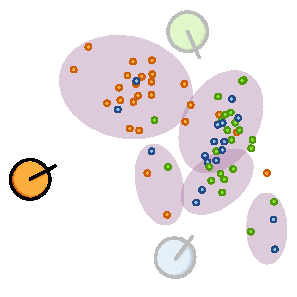
\includegraphics[width=3.3cm]{Figures/Mamot-1}
				};
				\node at (0,-3.5) [draw=black,ultra thick,inner sep=0pt]
				{
					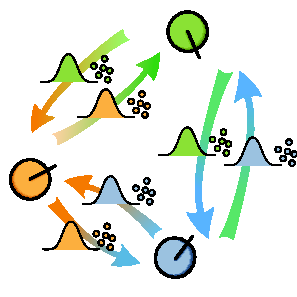
\includegraphics[width=3.3cm]{Figures/Mamot-2}
				};
			\end{tikzpicture}
		}
		
		\only<2->
		{
			\begin{algorithm}[H]
				\tiny
				\KwIn{perceptions $ z_{s,t} $, local track numbers $ oi_{s,t-1} $, global track numbers $ OI_{s,t-1} $}
				\BlankLine
				\KwData{set of local particles $ \tilde{\xi}_{s,t} $, set of global particles $ \tilde{\xi}_{\mathcal{S'},t} $, sensor pose $ m_{s,t} $, local GMM set $ \mathcal{L} $, global GMM set $ \mathcal{G} $}
				\BlankLine
				\KwOut{global estimations $ x_{s,t} = (\boldsymbol{OI}_{s,t},\boldsymbol\Lambda_{s,t},\boldsymbol{M}_{s,t},\boldsymbol\Sigma_{s,t}) $}
				\BlankLine
				\Begin
				{
					$ \tilde{\xi}_{s,t} \sim \pi_t (x_{s,t} | x_{s,t-1},z_{s,t},m_{s,t}) $
					\BlankLine
					Re-sample by using the SIR principle\\
					\BlankLine
					$ \mathcal{L} = KClusterize(\tilde{\xi}_{s,t}) $
					\BlankLine
					$ (\boldsymbol{oi}_{s,t},\boldsymbol\lambda_{s,t},\boldsymbol\mu_{s,t},\boldsymbol\sigma_{s,t}) = DataAssociation(\mathcal{L}, oi_{s,t-1}) $
					\BlankLine
					Communicate belief $ (\boldsymbol{oi}_{s,t},\boldsymbol\lambda_{s,t},\boldsymbol\mu_{s,t},\boldsymbol\sigma_{s,t}) $ to other agents
				}
				\BlankLine
				\Begin
				{
					\textcolor{lightred}{Collect $ \mathcal{L}_{S'} $ from a subset $ \mathcal{S'} \subseteq \mathcal{S} $ of sensors within a $ \Delta t $}
					\BlankLine
					\textcolor{lightred}{$ \tilde{\xi}_{\mathcal{S'},t} \sim \tilde\pi = \sum_{s \in \mathcal{S'}} \boldsymbol\lambda_{s,t} \, \mathcal{N} (\boldsymbol\mu_{s,t},\boldsymbol\sigma_{s,t}) $}
					\BlankLine
					\textcolor{lightred}{Re-sample by using the SIR principle}\\
					\BlankLine
					\textcolor{lightred}{$ \mathcal{G} = KClusterize(\tilde\xi_{{\mathcal{S'},t}}) $}
					\BlankLine
					\textcolor{lightred}{$ (\boldsymbol{OI}_{s,t},\boldsymbol\Lambda_{s,t},\boldsymbol{M}_{s,t},\boldsymbol\Sigma_{s,t}) = DataAssociation(\mathcal{G},OI_{s,t-1}) $}
				}
			\end{algorithm}
			
			\column{.01\textwidth}
			
			\Huge
			\vspace{2.15cm}
			
			\begin{center}
				\textcolor{blue}{$ \Rightarrow $}
			\end{center}
			
			\column{.44\textwidth}
			
			\centering
			
			\begin{tikzpicture}
				\node at (0,0) [draw=black,ultra thick,inner sep=0pt]
				{
					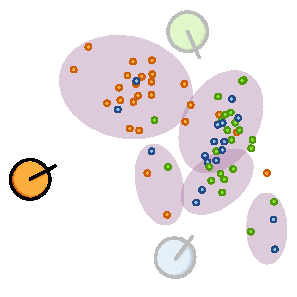
\includegraphics[width=3.3cm]{Figures/Mamot-1}
				};
				\node at (0,-3.5) [draw=black,ultra thick,inner sep=0pt]
				{
					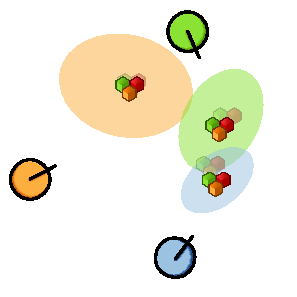
\includegraphics[width=3.3cm]{Figures/Mamot-3}
				};
			\end{tikzpicture}
		}
	\end{columns}
\end{frame}

\begin{frame}
	\frametitle{PTracking}
	\framesubtitle{Group Tracking}
	
	\begin{figure}
		\begin{tikzpicture}[map/.style={draw=black,ultra thick,inner sep=0pt}]
			\node at (0,0) [map] {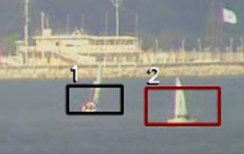
\includegraphics[width=0.32\linewidth]{Figures/GroupTracking-a}};
			\node at (4,0) [map] {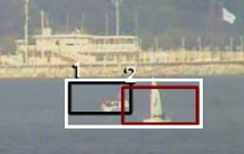
\includegraphics[width=0.32\linewidth]{Figures/GroupTracking-b}};
			\node at (8,0) [map] {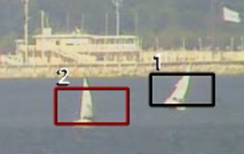
\includegraphics[width=0.32\linewidth]{Figures/GroupTracking-c}};
		\end{tikzpicture}
		\caption{Group tracking. Two sailing boats are going to cross each other. Occlusions are handled
				 considering the collapsing tracks to form a group, instead of tracking them
				 separately.}
	\end{figure}
\end{frame}

\begin{frame}
	\frametitle{KClusterize}
	\framesubtitle{Contributions}
	
	\Large
	
	\emph{KClusterize} has been designed aiming at fulfilling the following three requirements:
	
	\begin{enumerate}
		\item \textbf{Number} of objects to be detected \textbf{cannot} be known a priori
		\item \textbf{Low} computational load for real-time applications
		\item \textbf{Gaussian distribution} for each cluster
	\end{enumerate}
\end{frame}

\begin{frame}
	\frametitle{KClusterize}
	\framesubtitle{Typical Clustering Scenario}
	
	\vspace{0.5cm}
	
	\begin{figure}[!t]
		\begin{minipage}[l]{0.23\textwidth}
			\vspace*{\fill}
			\centering
			\subfigure[Analysed situation.]
			{
				\begin{tikzpicture}[map/.style={draw=white,ultra thick,inner sep=0pt}]
					\node at (0,0) [map]
					{
						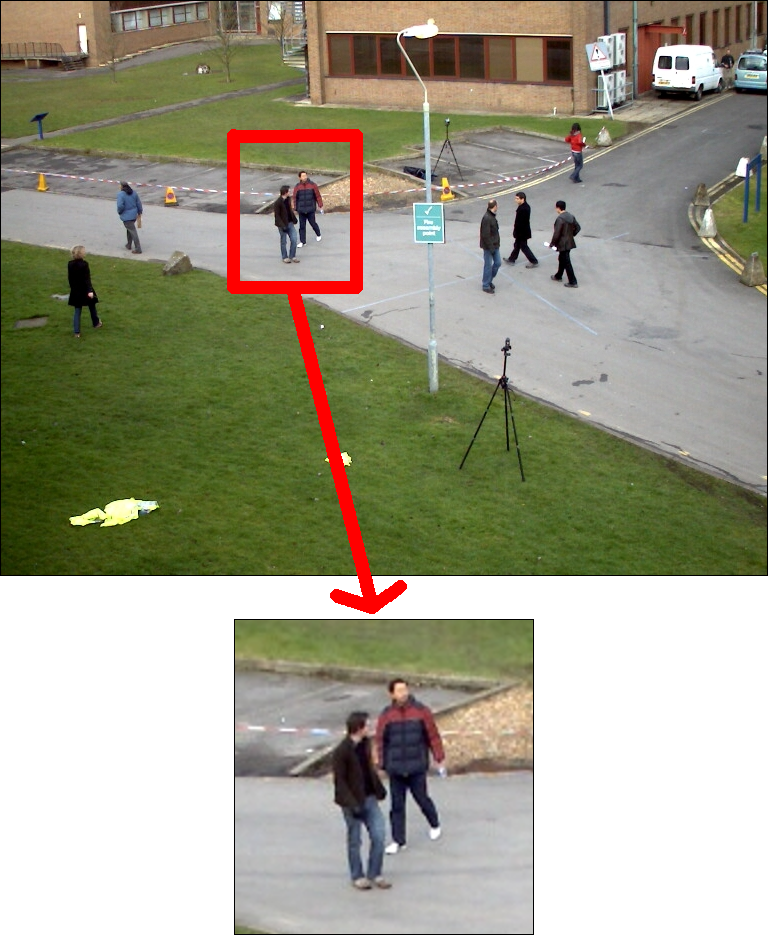
\includegraphics[width=\linewidth]{Figures/PETS-2009-Frame-0722-zoomed}
					};
				\end{tikzpicture}
			}
		\end{minipage}
		\hspace{0.1cm}
		\begin{minipage}[c]{0.74\textwidth}
			\subfigure[K-means with $ k = 2 $.]
			{
				\begin{tikzpicture}[map/.style={draw=white,ultra thick,inner sep=0pt}]
					\node at (0,0) [map]
					{
						\includegraphics[width=0.47\linewidth]{Figures/Kmeans-2.png}
					};
				\end{tikzpicture}
			}
			\hspace{-3.8mm}
			\subfigure[Hierarchical Clustering.]
			{
				\begin{tikzpicture}[map/.style={draw=white,ultra thick,inner sep=0pt}]
					\node at (0,0) [map]
					{
						\includegraphics[width=0.47\linewidth]{Figures/HierarchicalClustering.png}
					};
				\end{tikzpicture}
			}
			
			\subfigure[QT-Clustering.]
			{
				\begin{tikzpicture}[map/.style={draw=white,ultra thick,inner sep=0pt}]
					\node at (0,0) [map]
					{
						\includegraphics[width=0.47\linewidth]{Figures/QT-Clustering.png}
					};
				\end{tikzpicture}
			}
			\hspace{-3.8mm}
			\subfigure[KClusterize.]
			{
				\begin{tikzpicture}[map/.style={draw=white,ultra thick,inner sep=0pt}]
					\node at (0,0) [map]
					{
						\includegraphics[width=0.47\linewidth]{Figures/KClusterize.png}
					};
				\end{tikzpicture}
			}
		\end{minipage}
	\end{figure}
\end{frame}

\begin{frame}
	\frametitle{KClusterize}
	\framesubtitle{Clustering Speed}
	
	\begin{figure}[t]
		\begin{tikzpicture}[map/.style={draw=white,ultra thick,inner sep=0pt}]
			\node at (0,0) [map]
			{
				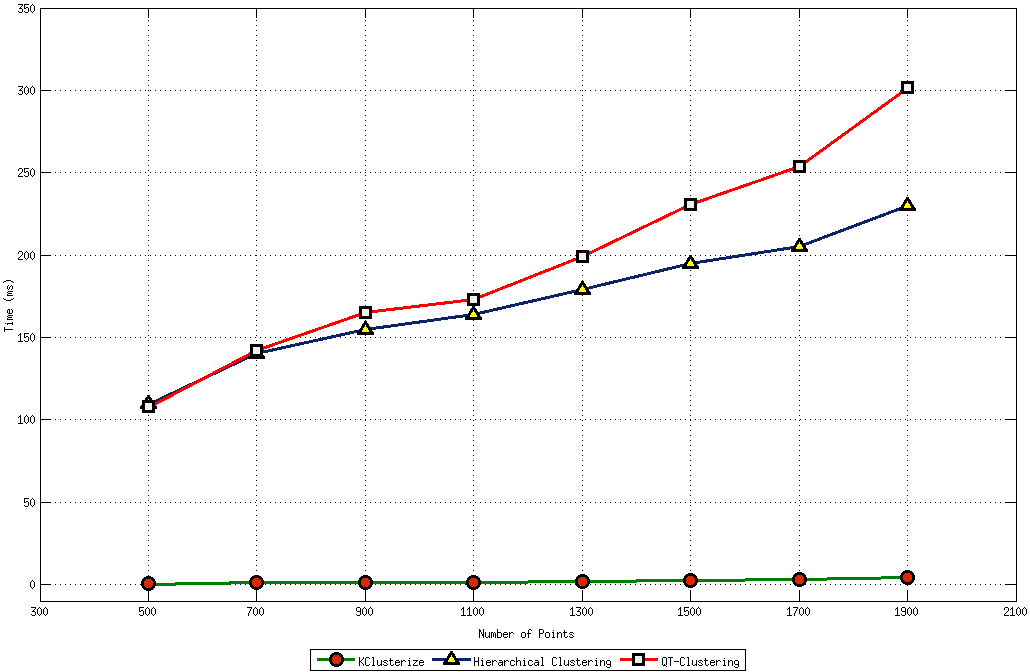
\includegraphics[width=0.88\linewidth]{Figures/ClusteringComparison}
			};
		\end{tikzpicture}
	\end{figure}
\end{frame}

\begin{frame}
	\frametitle{KClusterize}
	\framesubtitle{Cluster Gaussian Distribution}
	
	\vspace{0.3cm}
	
	\setcounter{subfigure}{0}
	
	\begin{figure}[!t]
		\centering
		\subfigure[Output of the algorithm on frame \#269.]
		{
			\begin{tikzpicture}[map/.style={draw=black,ultra thick,inner sep=0pt}]
				\node at (0,0) [map]
				{
					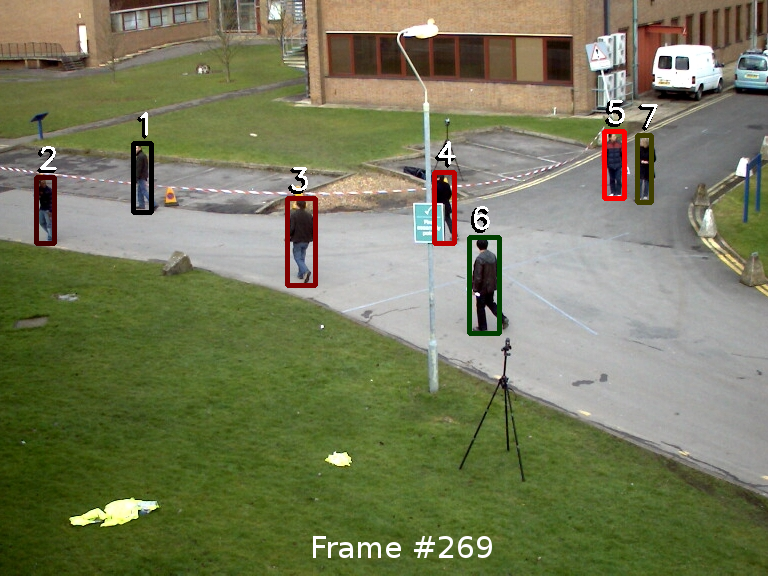
\includegraphics[width=0.48\linewidth]{Figures/KClusterize-Frame-0269-Output.png}
				};
			\end{tikzpicture}
		}
		\hspace{-3.8mm}
		\subfigure[A 2D visualization of frame \#269.]
		{
			\begin{tikzpicture}[map/.style={draw=white,ultra thick,inner sep=0pt}]
				\node at (0,0) [map]
				{
					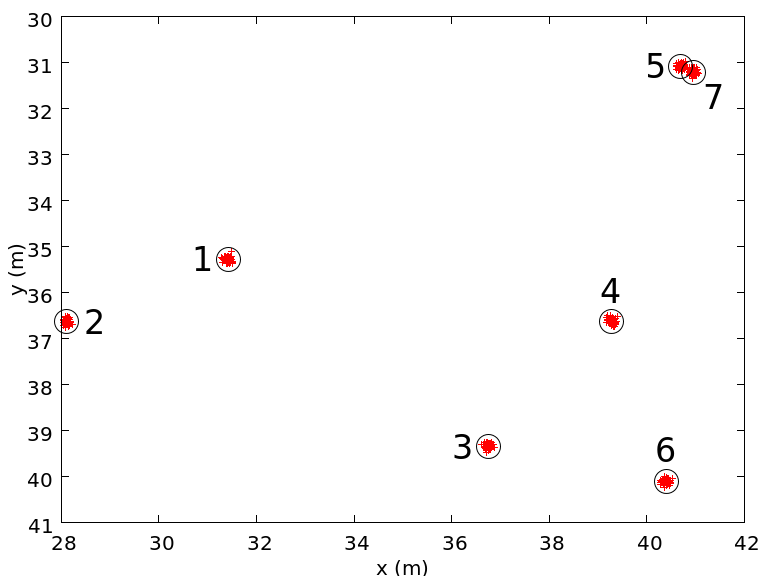
\includegraphics[width=0.48\linewidth]{Figures/KClusterize-Frame-0269-PlaneView.png}
				};
			\end{tikzpicture}
		}
	\end{figure}
\end{frame}

\section{Experimental Evaluation - Tracking}

\begin{frame}
	\frametitle{Evaluating a Tracking Algorithm}
	
	\Large
	
	\vspace{0.45cm}
	
	The CLEAR MOT (Kasturi et al. \cite{Kasturi09}) metrics \emph{MOTA} and \emph{MOTP} are the
	de-facto standard for evaluating a tracking method:
	
	\vspace{-0.5cm}
	
	\begin{equation*}
		MOTA = 1 - \frac{\sum_{t=1}^{N_{frames}} \big [ c_m(m_t) + c_f(fp_t) + cs(ID\mbox{-}S_t) \big ]}{\sum_{t=1}^{N_{frames}} N_G^{(t)}}
	\end{equation*}
	
	\vspace{0.4cm}
	
	\begin{equation*}
		MOTP = \frac{\sum_{i=1}^{N_{mapped}} \sum_{t=1}^{N_{frames}^{(t)}} \Big [ \frac{| G_i^{(t)} \cap D_i^{(t)} |}{| G_i^{(t)} \cup D_i^{(t)} |} \Big ] }{\sum_{t=1}^{N_{frames}} N_{mapped}^{(t)}}
	\end{equation*}
	
	\vspace{0.3cm}
	
	\tiny
	
	\cite{Kasturi09} R. Kasturi \emph{et al.},  ``Framework for performance evaluation of face, text,
	and vehicle detection and tracking in video: data,\\ \hspace{0.25cm} metrics, and protocol'', PAMI,
	2009 \\
\end{frame}

\begin{frame}
	\frametitle{Experimental Evaluation}
	\framesubtitle{Single-Sensor, Multi-Object}
	
	\large
	
	\begin{columns}[t]
		\only<1->
		{
			\column{0.8\textwidth}
			
			\begin{block}{Boat Visual Tracking}
				automatic surveillance system in the maritime domain
			\end{block}
			
			\column{0.15\textwidth}
		}
	\end{columns}
	
	\vspace{0.3cm}
	
	\begin{center}
		\begin{tikzpicture}
			\node at (0,0) [draw=black,ultra thick,inner sep=0pt]  {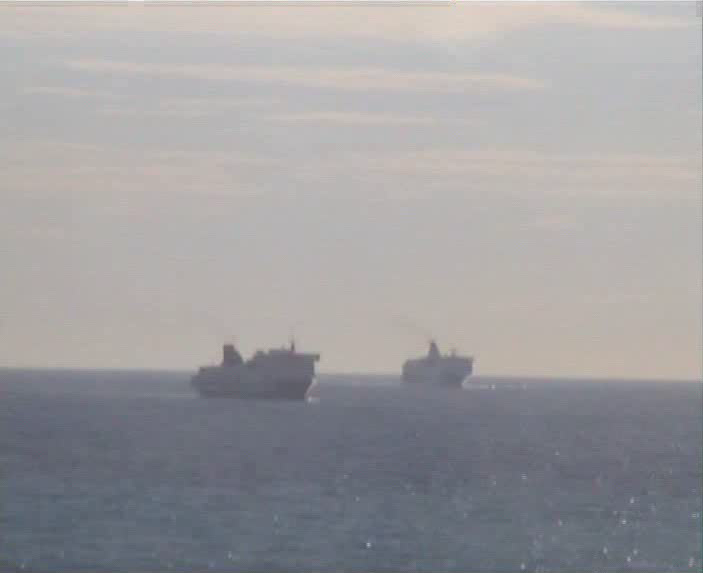
\includegraphics[height=3.1cm]{Figures/Boat-1}};
			\node at (3.95,0) [draw=black,ultra thick,inner sep=0pt]  {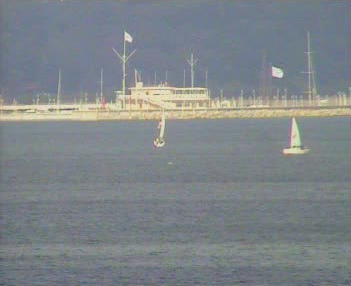
\includegraphics[height=3.1cm]{Figures/Boat-2}};
			\node at (7.95,0) [draw=black,ultra thick,inner sep=0pt]  {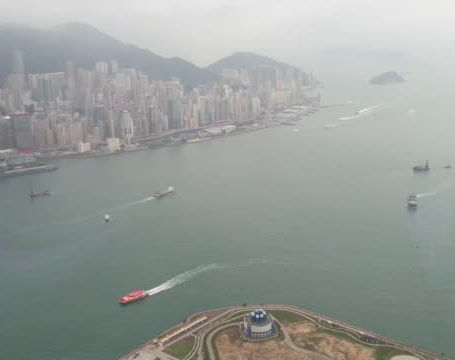
\includegraphics[height=3.1cm]{Figures/Boat-3}};
		\end{tikzpicture}
	\end{center}
	
	\vspace{0.45cm}
	
	\tiny
	
	\textbf{Enhancing Automatic Maritime Surveillance Systems with Visual Information} \\
	D. D. Bloisi, F. Previtali, A. Pennisi, D. Nardi, M. Fiorini \\
	\emph{IEEE Transaction on Intelligent Transportation Systems} [second revision] \\
\end{frame}

\begin{frame}
	\frametitle{Quantitative Evaluation}
	\framesubtitle{Maritime Domain}
	
	\large
	
	\begin{table}[!t]
		\renewcommand{\arraystretch}{1.3}
		\caption{\large Tracking performance on the maritime domain. MOTA (higher the better) considers
				 the number of missed detections, the number of false positives and the switches of
				 identities. MOTP (higher the better) considers the precision of the detections.}
		\centering
		\vspace{0.2cm}
		
		\begin{tabular}{ccc}
			\hline
			\hline
			\textbf{Video} & \textbf{MOTA} & \textbf{MOTP} \\
			\hline
			occlusions-1.avi & 0.815 & 0.613 \\
			\hline
			occlusions-2.avi & 0.910 & 0.554 \\
			\hline
			high-view.avi & 0.910 & 0.604 \\
			\hline
		\hline
		\end{tabular}
	\end{table}
\end{frame}

\begin{frame}
	\frametitle{Qualitative Evaluation}
	\framesubtitle{Maritime Domain - Blue Water}
	
	\begin{figure}[!h]
		\centering
		\includemovie[inline=false,text=
		{
			\begin{tikzpicture}
				\node at (0,0) [draw=black,ultra thick,inner sep=0pt]
				{
					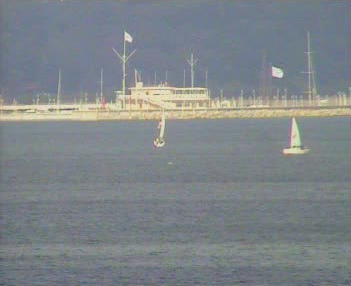
\includegraphics[width=0.65\linewidth]{Figures/Boat-2}
				};
			\end{tikzpicture}
		}]{}{}{../Videos/1-Boat/PTracking-Wester_LLTV_VELA.avi}
	\end{figure}
\end{frame}

\begin{frame}
	\frametitle{Qualitative Evaluation}
	\framesubtitle{Maritime Domain - Hong Kong Port}
	
	\begin{figure}[!h]
		\centering
		\includemovie[inline=false,text=
		{
			\begin{tikzpicture}
				\node at (0,0) [draw=black,ultra thick,inner sep=0pt]
				{
					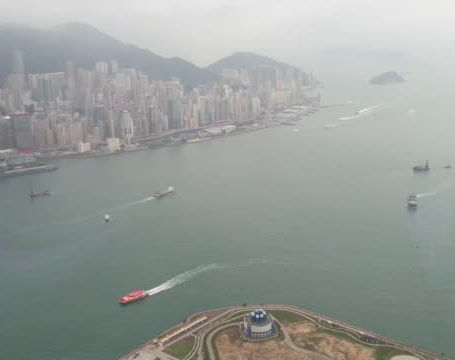
\includegraphics[width=0.65\linewidth]{Figures/Boat-3}
				};
			\end{tikzpicture}
		}]{}{}{../Videos/1-Boat/PTracking-Honk-Kong.avi}
	\end{figure}
\end{frame}

\begin{frame}
	\frametitle{Experimental Evaluation}
	\framesubtitle{Multi-Sensor, Single-Object}
	
	\large
	
	\vspace{-0.3cm}
	
	\begin{columns}[t]
		\only<1->
		{
			\column{0.8\textwidth}
			
			\begin{block}{Soccer Robots}
				used to solve the localisation field symmetry problem
			\end{block}
			
			\column{0.15\textwidth}
		}
	\end{columns}
	
	\vspace{0.15cm}
	
	\begin{center}
		\begin{tikzpicture}
			\node at (0,0) [draw=black,ultra thick,inner sep=0pt]
			{
				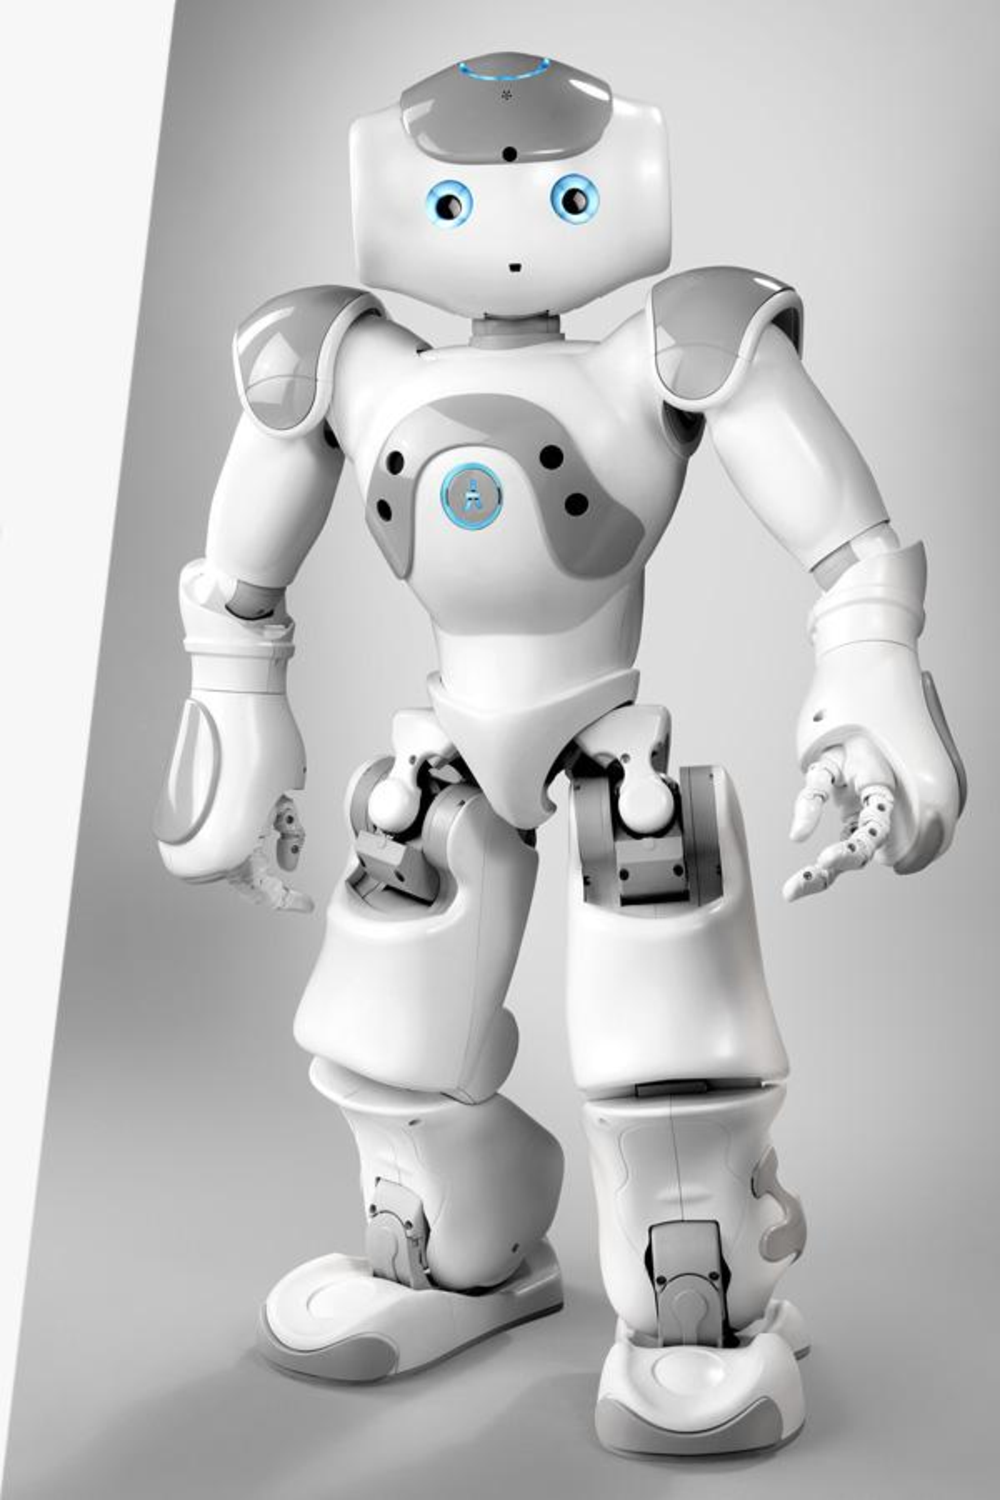
\includegraphics[scale=0.2]{Figures/Nao}
			};
		\end{tikzpicture}
	\end{center}
	
	\tiny
	
	\textbf{Disambiguating Localization Symmetry through a Multi-Clustered Particle Filtering} \\
	F. Previtali, G. Gemignani, L. Iocchi, D. Nardi \\
	\emph{IEEE International Conference on Multisensor Fusion and Integration for Intelligent Systems,
	2015} \\
\end{frame}

\begin{frame}
	\frametitle{Challenge}
	
	\Large
	
	\vspace{0.25cm}
	
	\begin{figure}
		\centering
		\begin{tikzpicture}
			\node at (0,0) [draw=white,ultra thick,inner sep=0pt]
			{
				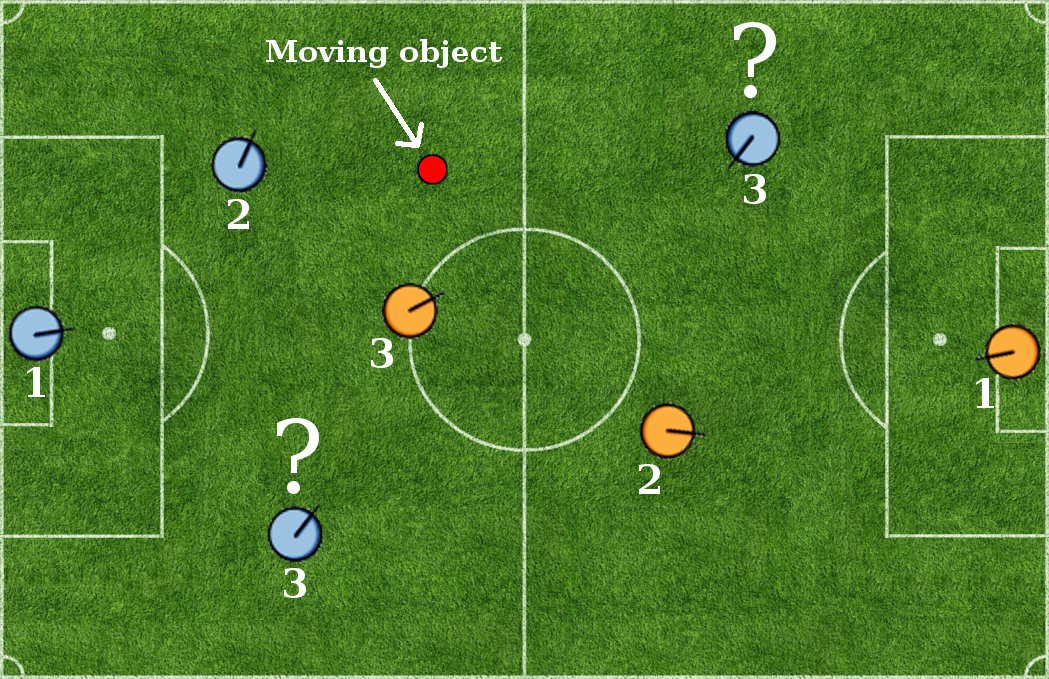
\includegraphics[width=0.8\linewidth]{Figures/Challenge}
			};
		\end{tikzpicture}
	\end{figure}
	
	\vspace{-0.4cm}
	
	\begin{center}
		What is the real position of the blue robot number 3?
	\end{center}
\end{frame}

\begin{frame}
	\frametitle{Quantitative Evaluation}
	\framesubtitle{RoboCup Domain}
	
	\large
	
	\vspace{-0.85cm}
	
	Simulating 3 Aldebaran Nao robots playing soccer, one of them alternatively forced to be inversely
	localised
	
	\Large
	
	\vspace{-0.6cm}
	
	\begin{columns}[T]
		\column{1.02\textwidth}
		
	\begin{figure}
		\centering
		
		\begin{tikzpicture}
			\node at (0,0) [draw=white,ultra thick,inner sep=0pt]
			{
				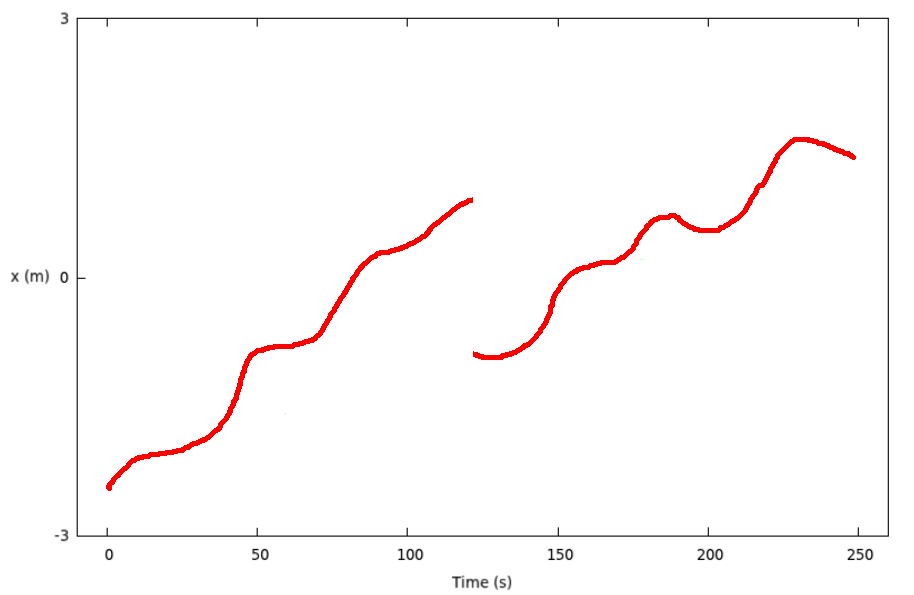
\includegraphics[width=0.34\linewidth]{Figures/Result-Scenario-2_Robot-1}
			};
			\node at (4.1,0) [draw=white,ultra thick,inner sep=0pt]
			{
				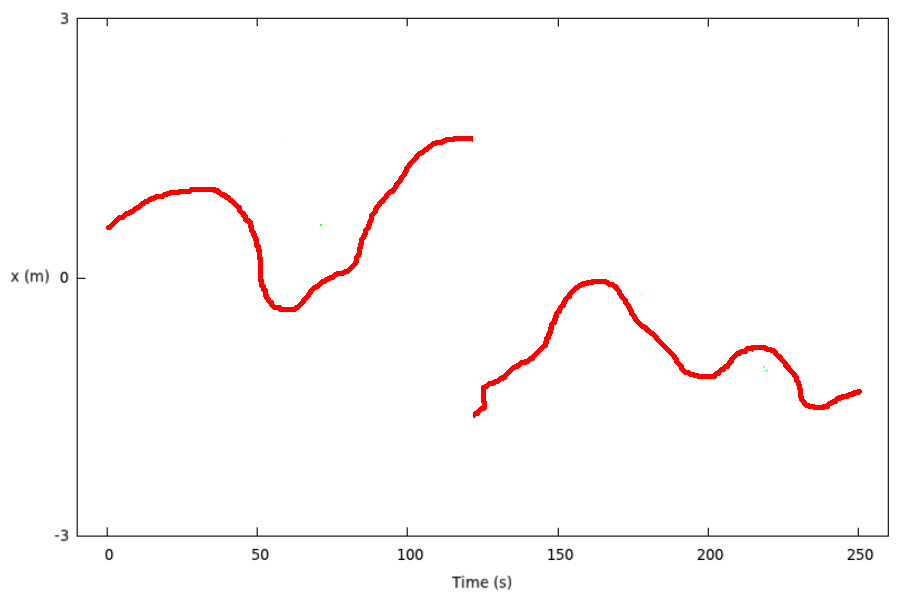
\includegraphics[width=0.34\linewidth]{Figures/Result-Scenario-2_Robot-2}
			};
			\node at (0,-2.9) [draw=white,ultra thick,inner sep=0pt]
			{
				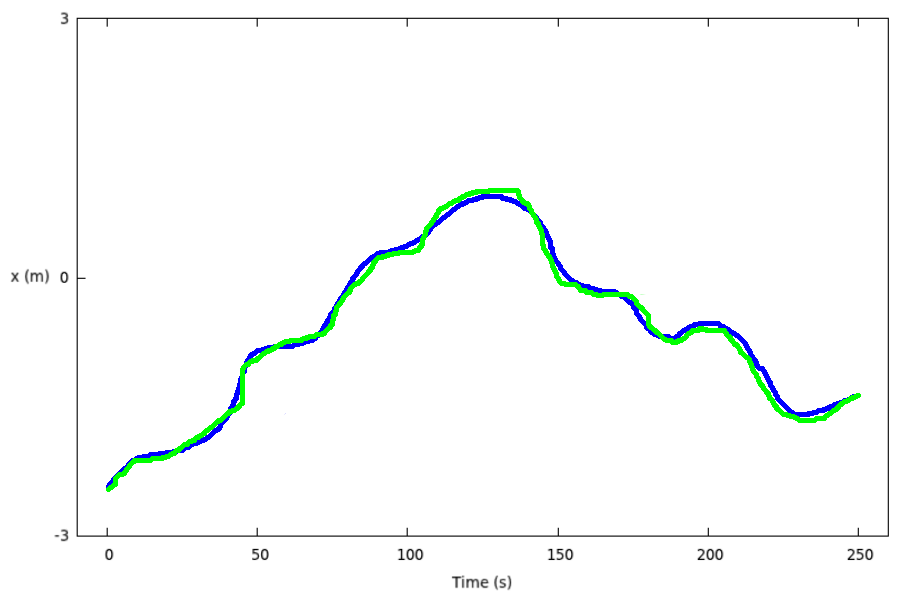
\includegraphics[width=0.34\linewidth]{Figures/Result-Scenario-2_Robot-1-GT}
			};
			\node at (4.1,-2.9) [draw=white,ultra thick,inner sep=0pt]
			{
				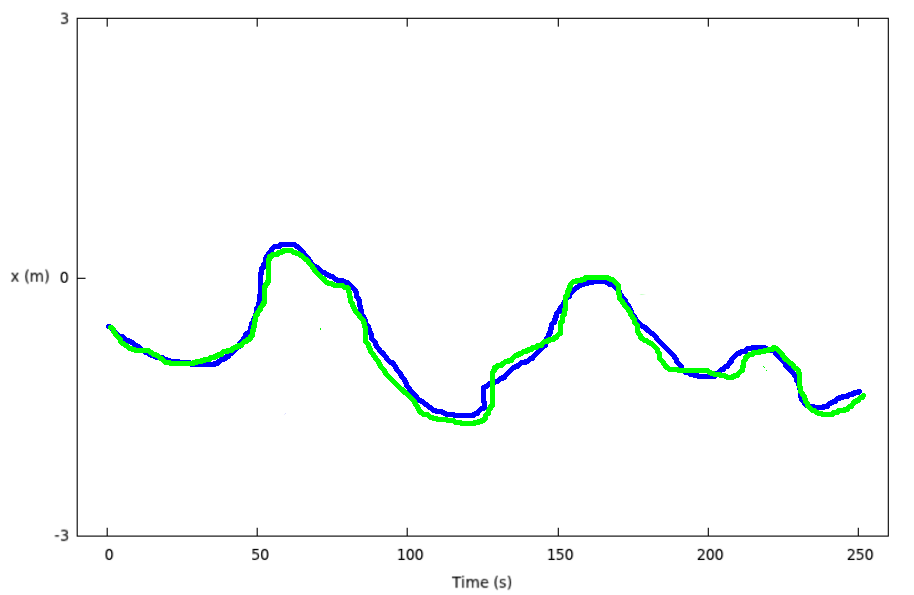
\includegraphics[width=0.34\linewidth]{Figures/Result-Scenario-2_Robot-2-GT}
			};
			\node at (8.2,0) [draw=white,ultra thick,inner sep=0pt]
			{
				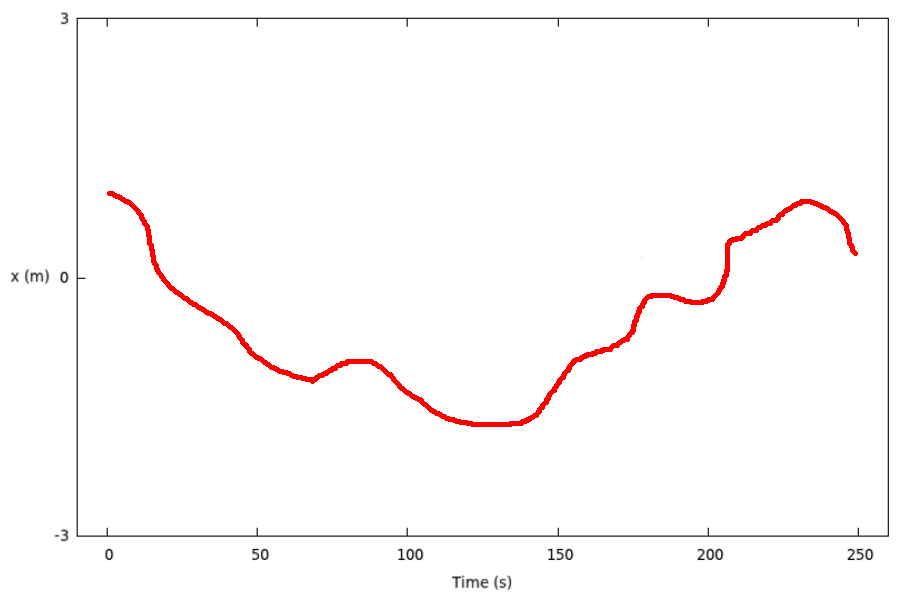
\includegraphics[width=0.34\linewidth]{Figures/Result-Scenario-2_Robot-3}
			};
			\node at (8.2,-2.9) [draw=white,ultra thick,inner sep=0pt]
			{
				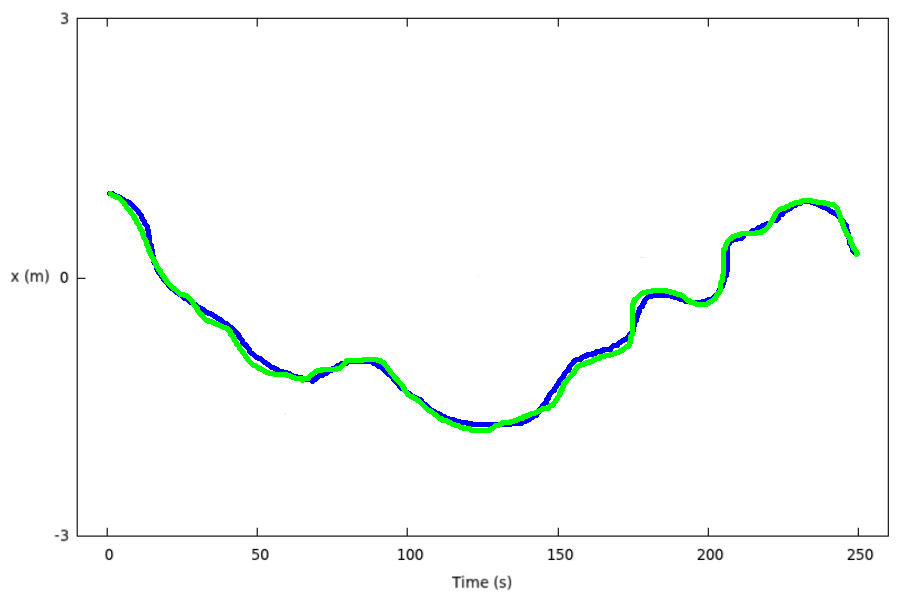
\includegraphics[width=0.34\linewidth]{Figures/Result-Scenario-2_Robot-3-GT}
			};
		\end{tikzpicture}
	\end{figure}
	\end{columns}
	
	\vspace{-6.15cm}
	
	\begin{tabbing}
		\hspace{0.21cm}
		\tiny
		\textbf{Robot 1 - Localization}
		\hspace{1.79cm}
		\textbf{Robot 2 - Localization}
		\hspace{1.79cm}
		\textbf{Robot 3 - Localization}
	\end{tabbing}
	
	\vspace{-1cm}
	
	\begin{tabbing}
		\hspace{0.4cm}
		\tiny
		\textcolor{blue}{Correctly}
	\end{tabbing}
	
	\vspace{-1.2cm}
	
	\begin{tabbing}
		\hspace{0.42cm}
		\tiny
		\textcolor{blue}{localized}
	\end{tabbing}
	
	\vspace{-1.17cm}
	
	\begin{tabbing}
		\footnotesize
		\hspace{0.87cm}
		\textcolor{blue}{$ \searrow $}
	\end{tabbing}
	
	\vspace{-1.43cm}
	
	\begin{tabbing}
		\footnotesize
		\hspace{2.68cm}
		\textcolor{blue}{$ \nwarrow $}
	\end{tabbing}
	
	\vspace{-1.2cm}
	
	\begin{tabbing}
		\hspace{2.53cm}
		\tiny
		\textcolor{blue}{Wrongly}
	\end{tabbing}
	
	\vspace{-1.2cm}
	
	\begin{tabbing}
		\hspace{2.52cm}
		\tiny
		\textcolor{blue}{localized}
	\end{tabbing}
	
	\vspace{-1.83cm}
	
	\begin{tabbing}
		\footnotesize
		\hspace{4.8cm}
		\textcolor{blue}{$ \nearrow $}
	\end{tabbing}
	
	\vspace{-1.2cm}
	
	\begin{tabbing}
		\hspace{4.35cm}
		\tiny
		\textcolor{blue}{Wrongly}
	\end{tabbing}
	
	\vspace{-1.2cm}
	
	\begin{tabbing}
		\hspace{4.34cm}
		\tiny
		\textcolor{blue}{localized}
	\end{tabbing}
	
	\vspace{-2.75cm}
	
	\begin{tabbing}
		\hspace{6.82cm}
		\tiny
		\textcolor{blue}{Correctly}
	\end{tabbing}
	
	\vspace{-1.2cm}
	
	\begin{tabbing}
		\hspace{6.84cm}
		\tiny
		\textcolor{blue}{localized}
	\end{tabbing}
	
	\vspace{-1.17cm}
	
	\begin{tabbing}
		\footnotesize
		\hspace{7cm}
		\textcolor{blue}{$ \swarrow $}
	\end{tabbing}
	
	\vspace{-1.79cm}
	
	\begin{tabbing}
		\hspace{9.52cm}
		\tiny
		\textcolor{blue}{Correctly}
	\end{tabbing}
	
	\vspace{-1.2cm}
	
	\begin{tabbing}
		\hspace{9.54cm}
		\tiny
		\textcolor{blue}{localized}
	\end{tabbing}
	
	\vspace{-1.17cm}
	
	\begin{tabbing}
		\footnotesize
		\hspace{9.99cm}
		\textcolor{blue}{$ \searrow $}
	\end{tabbing}
	
	\vspace{0.01cm}
	
	\begin{tabbing}
		\hspace{0.21cm}
		\tiny
		\textbf{Robot 1 - Filtered vs Ground-Truth}
		\hspace{0.53cm}
		\textbf{Robot 2 - Filtered vs Ground-Truth}
		\hspace{0.53cm}
		\textbf{Robot 3 - Filtered vs Ground-Truth}
	\end{tabbing}
\end{frame}

\begin{frame}
	\frametitle{Qualitative Evaluation}
	\framesubtitle{RoboCup Iran Open}
	
	\begin{figure}[!h]
		\centering
		\includemovie[inline=false,text=
		{
			\begin{tikzpicture}
				\node at (0,0) [draw=black,ultra thick,inner sep=0pt]
				{
					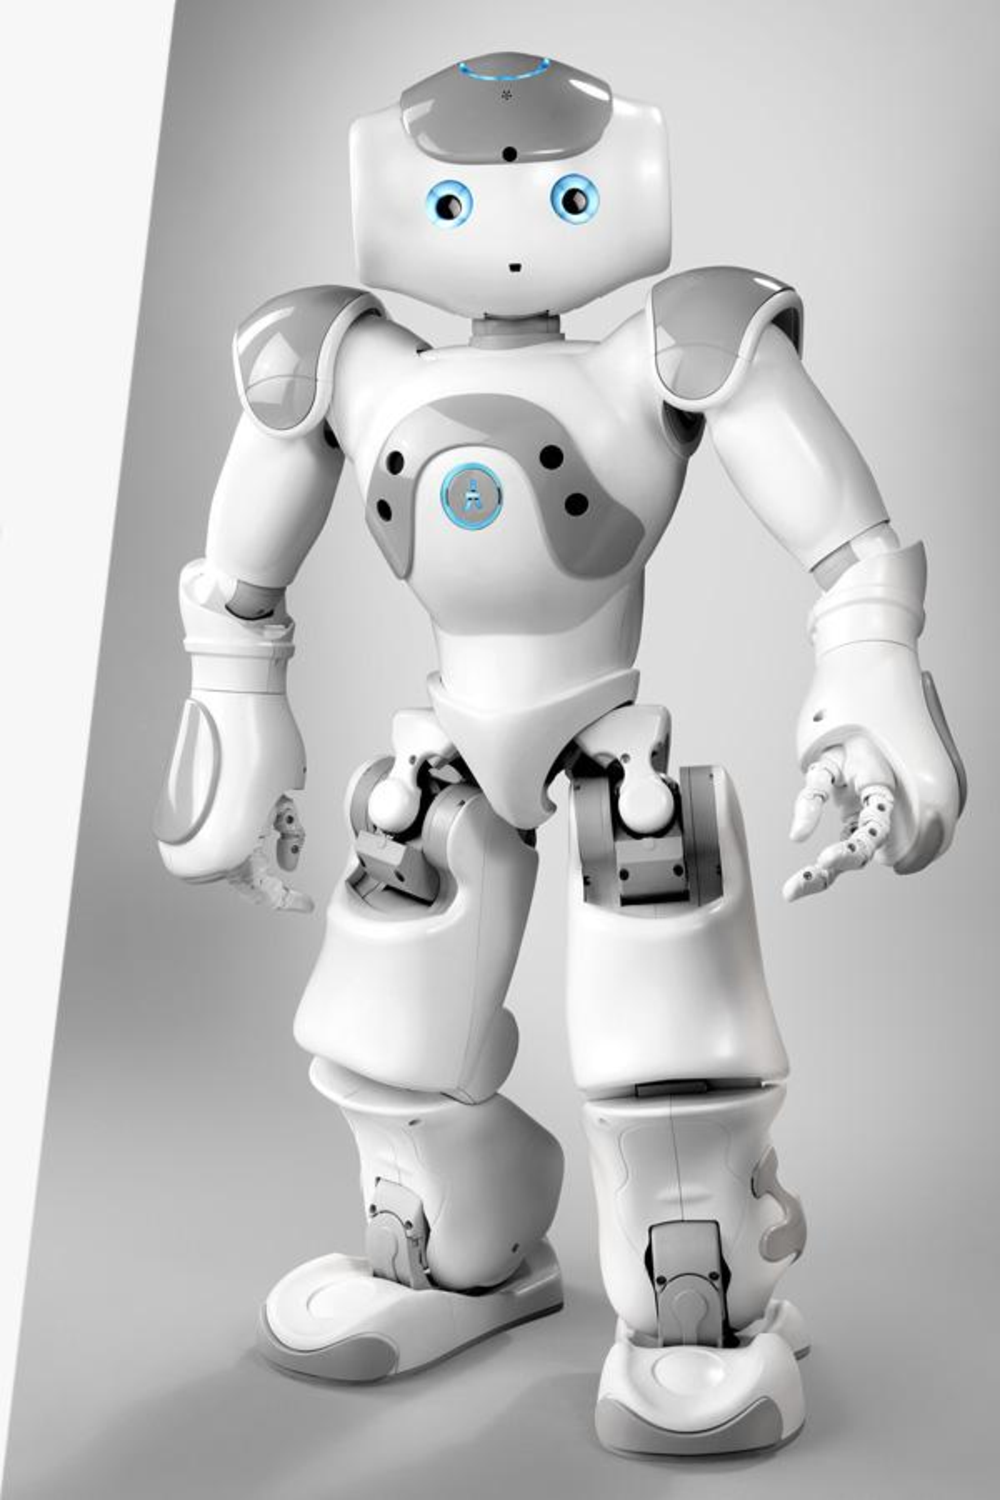
\includegraphics[width=0.85\linewidth]{Figures/Nao}
				};
			\end{tikzpicture}
		}]{}{}{../Videos/2-Nao/PTracking-RLSD.avi}
	\end{figure}
\end{frame}

\begin{frame}
	\frametitle{Experimental Evaluation}
	\framesubtitle{Multi-Sensor, Multi-Object}
	
	\large
	
	\vspace{-0.35cm}
	
	\begin{columns}[t]
		\only<1->
		{
			\column{0.8\textwidth}
			
			\begin{block}{Issia Soccer}
				tracking of players in a real soccer match
			\end{block}
			
			\column{0.15\textwidth}
		}
	\end{columns}
	
	\begin{center}
		\begin{tikzpicture}
			\node at (2.39,0) [draw=black,ultra thick,inner sep=0pt]  {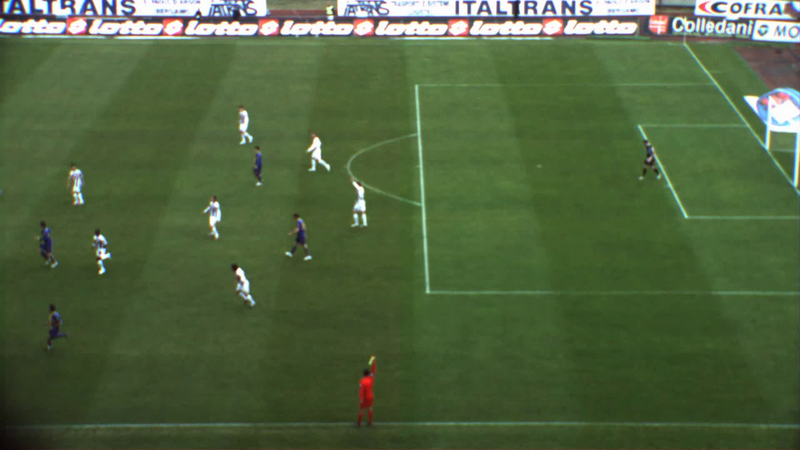
\includegraphics[height=2.1cm]{Figures/IssiaSoccer-Camera1}};
			\node at (6.26,0) [draw=black,ultra thick,inner sep=0pt]  {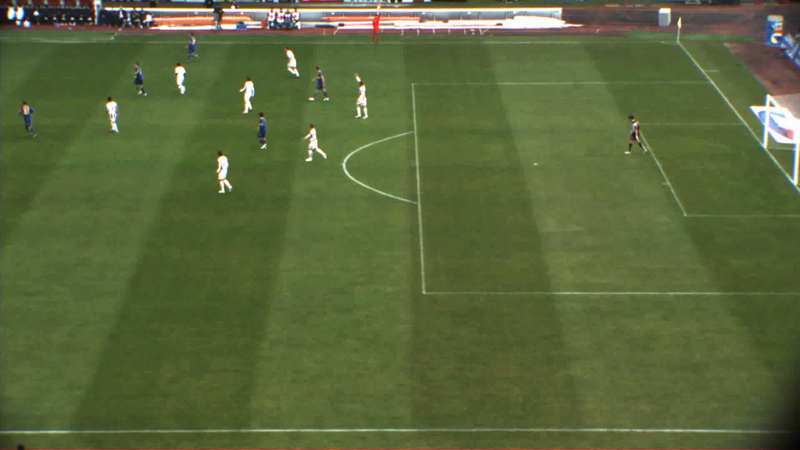
\includegraphics[height=2.1cm]{Figures/IssiaSoccer-Camera2}};
			\node at (2.39,-2.22) [draw=black,ultra thick,inner sep=0pt]  {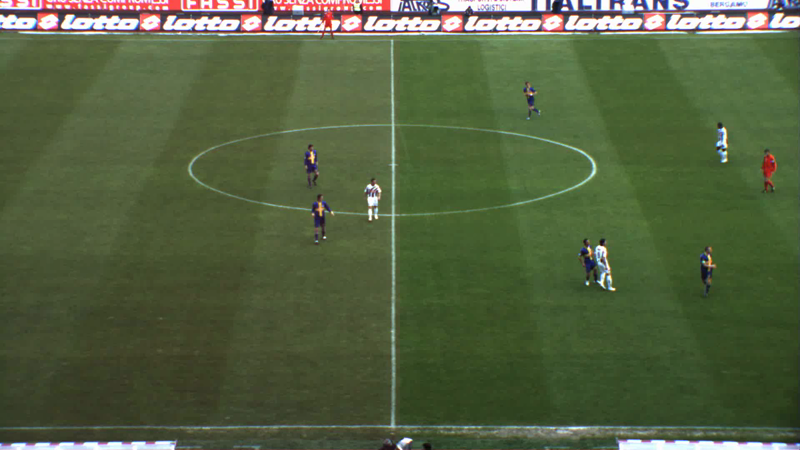
\includegraphics[height=2.1cm]{Figures/IssiaSoccer-Camera3}};
			\node at (6.26,-2.22) [draw=black,ultra thick,inner sep=0pt]  {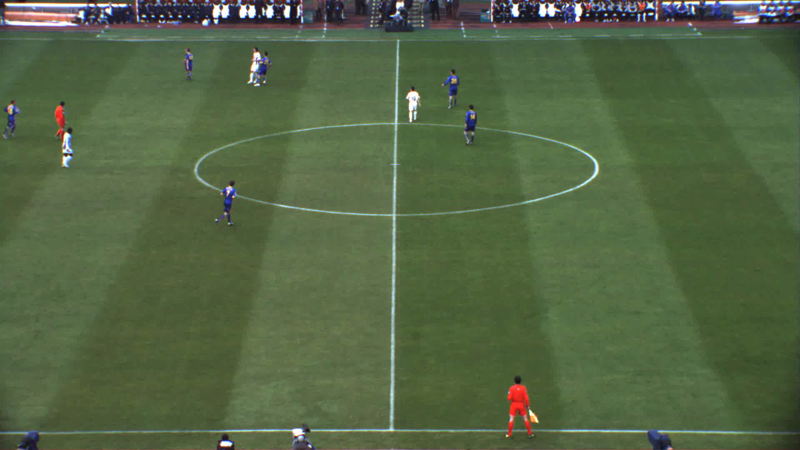
\includegraphics[height=2.1cm]{Figures/IssiaSoccer-Camera4}};
		\end{tikzpicture}
	\end{center}
	
	\vspace{-0.05cm}
	
	\tiny
	
	\textbf{A Distributed Approach for Real-Time Multi-Camera Multi-Object Tracking} \\
	F. Previtali, D. D. Bloisi, L. Iocchi \\
	\emph{Journal on Computer Vision and Image Understanding} [second revision] \\
\end{frame}

\begin{frame}
	\frametitle{Quantitative Evaluation}
	\framesubtitle{People Domain - Issia Soccer}
	
	\Large
	
	\begin{table}[!t]
		\renewcommand{\arraystretch}{1.3}
		\centering
		\begin{tabular}{lcccc}
			\hline
			\hline
			\multicolumn{1}{c}{\begin{tabular}[c]{@{}c@{}}\textbf{Method} \end{tabular}} & \textbf{MOTA} & \textbf{MOTP} \\
			\hline
			PTracking - Camera 1 & 0.723 & 0.612 \\
			\hline
			PTracking - Camera 1, 2 & 0.789 & 0.638 \\
			\hline
			PTracking - Camera 1, 2, 3 & 0.817 & 0.651 \\
			\hline
			PTracking - Camera 1, 2, 3, 4 & 0.894 & 0.706 \\
			\hline
		\hline
		\end{tabular}
	\end{table}
\end{frame}

\begin{frame}
	\frametitle{Qualitative Evaluation}
	\framesubtitle{People Domain - Issia Soccer}
	
	\begin{figure}[!h]
		\centering
		\includemovie[inline=false,text=
		{
			\begin{tikzpicture}
				\node at (0,0) [draw=black,ultra thick,inner sep=0pt]
				{
					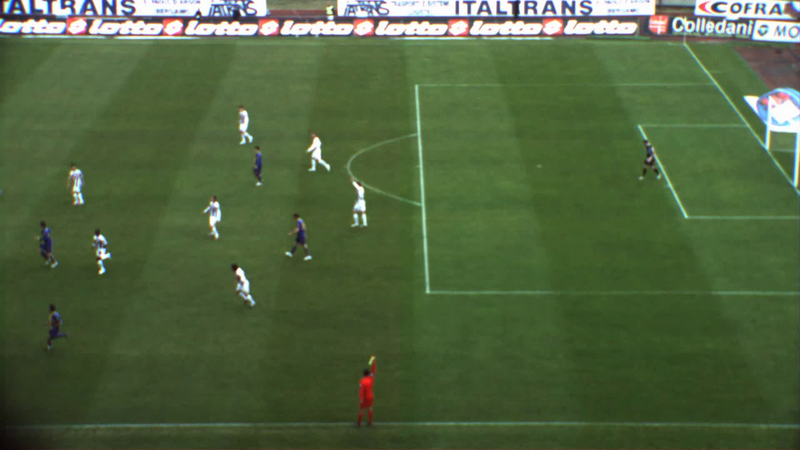
\includegraphics[width=0.85\linewidth]{Figures/IssiaSoccer-Camera1}
				};
			\end{tikzpicture}
		}]{}{}{../Videos/4-People/PTracking-IssiaSoccer.mp4}
	\end{figure}
\end{frame}

\begin{frame}
	\frametitle{Experimental Evaluation}
	\framesubtitle{Multi-Sensor, Multi-Object}
	
	\large
	
	\vspace{-0.45cm}
	
	\begin{columns}[t]
		\only<1->
		{
			\column{0.8\textwidth}
			
			\begin{block}{PETS-2009}
				tracking of individuals within a crowd
			\end{block}
			
			\column{0.15\textwidth}
		}
	\end{columns}
	
	\vspace{0.1cm}
	
	\begin{center}
		\begin{tikzpicture}
			\node at (0,0) [draw=black,ultra thick,inner sep=0pt]  {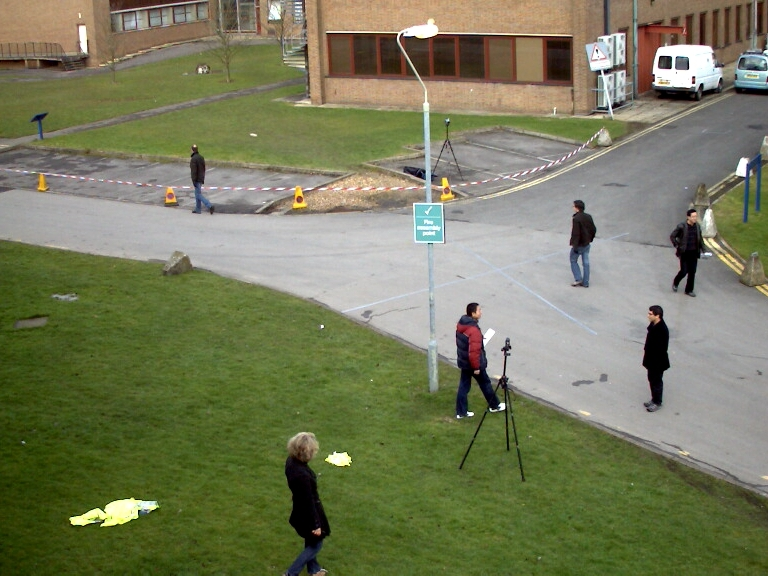
\includegraphics[height=2.55cm]{Figures/PETS2009-1}};
			\node at (3.55,0) [draw=black,ultra thick,inner sep=0pt]  {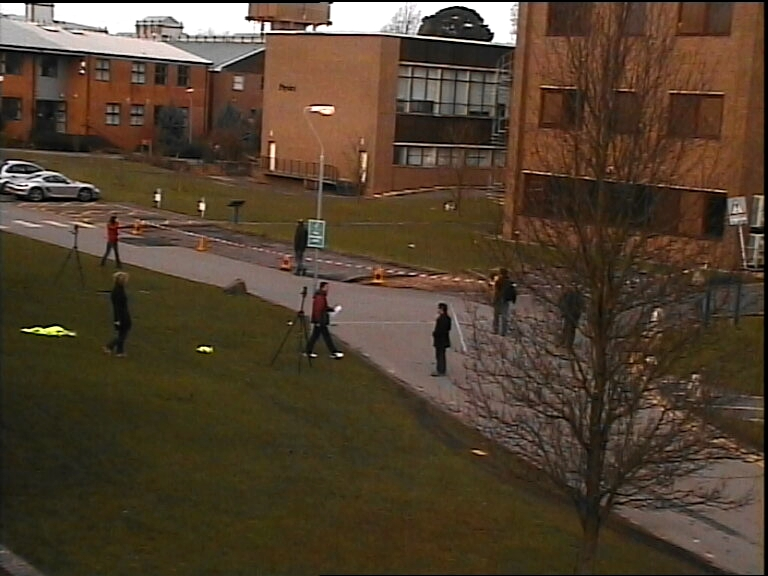
\includegraphics[height=2.55cm]{Figures/PETS2009-3}};
			\node at (7.17,0) [draw=black,ultra thick,inner sep=0pt]  {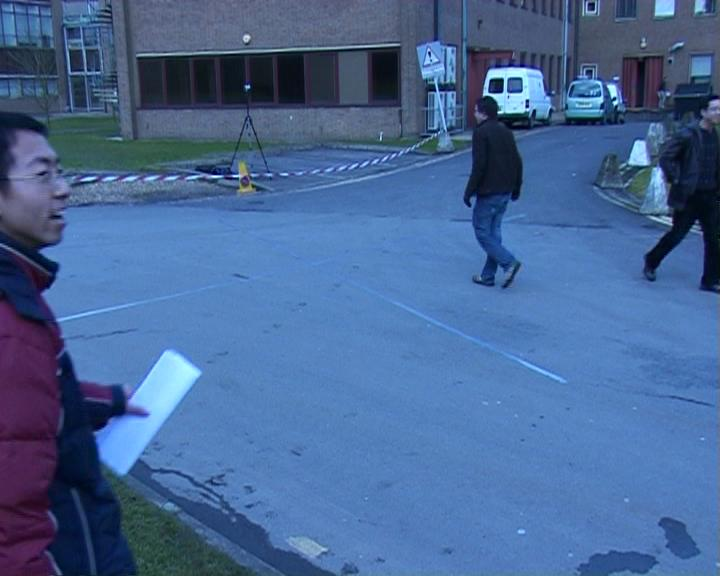
\includegraphics[height=2.55cm]{Figures/PETS2009-6}};
			\node at (1.8,-2.7) [draw=black,ultra thick,inner sep=0pt]  {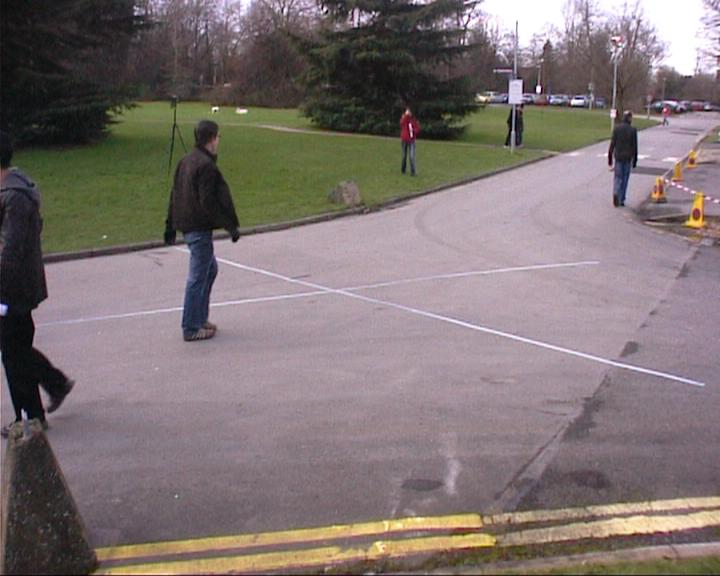
\includegraphics[height=2.55cm]{Figures/PETS2009-7}};
			\node at (5.5,-2.7) [draw=black,ultra thick,inner sep=0pt]  {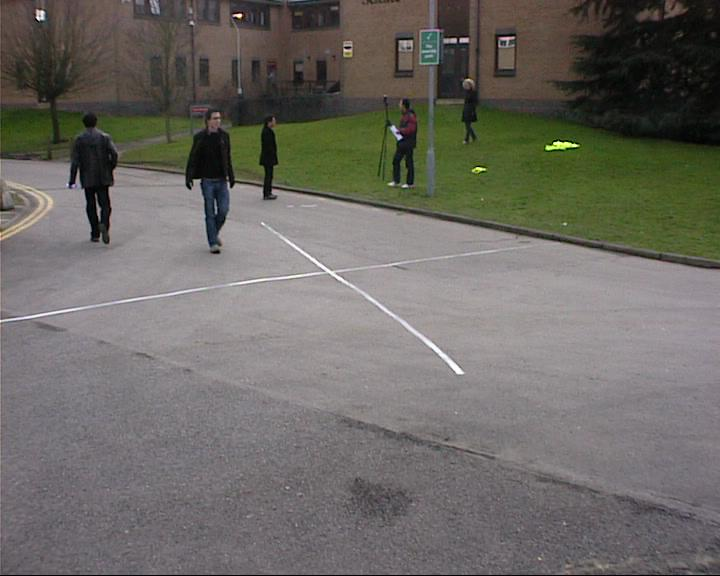
\includegraphics[height=2.55cm]{Figures/PETS2009-8}};
		\end{tikzpicture}
	\end{center}
\end{frame}

\begin{frame}
	\frametitle{Quantitative Evaluation}
	\framesubtitle{People Domain - PETS-2009}
	
	\large
	
	\begin{table}[!t]
		\renewcommand{\arraystretch}{1.3}
		\centering
		\begin{tabular}{ccccc}
			\hline
			\hline
			\textbf{Method} & \textbf{MOTA} & \textbf{MOTP} & \textbf{Type} & \textbf{Real-Time} \\
			\hline
			Leal-Taix\'{e} \cite{Leal11} & 0.67 & 0.534 & OFFLINE & NO \\
			\hline
			Berclaz \cite{Berclaz11} & 0.732 & 0.603 & OFFLINE & NO \\
			\hline
			Henriques \cite{Henriques11} & 0.833 & 0.711 & OFFLINE & NO \\
			\hline
			Breitenstein \cite{Breitenstein11} & 0.745 & 0.563 & ONLINE & NO \\
			\hline
			Yang \cite{Yang09} & 0.759 & 0.538 & ONLINE & NO \\
			\hline
			Bae \cite{Bae14} & 0.830 & 0.696 & ONLINE & \textbf{YES} \\
			\hline
			PTracking & \textbf{0.874} & \textbf{0.722} & ONLINE & \textbf{YES (30.2 FPS)} \\
			\hline
			PTracking$^*$ & \textbf{0.882} & \textbf{0.717} & ONLINE & NO (11.8 FPS) \\
			\hline
		\hline
		\end{tabular}
	\end{table}
\end{frame}

\begin{frame}
	\frametitle{Experimental Evaluation}
	\framesubtitle{Multi-Sensor, Multi-Object}
	
	\large
	
	\begin{columns}[t]
		\only<1->
		{
			\column{0.8\textwidth}
			
			\begin{block}{Prey-Predator Game}
				demonstrating the advantages of using mobile sensors
			\end{block}
			
			\column{0.15\textwidth}
		}
	\end{columns}
	
	\vspace{0.1cm}
	
	\begin{center}
		\begin{tikzpicture}
			\node at (0,0) [draw=black,ultra thick,inner sep=0pt]  {\includegraphics[height=3.25cm]{Figures/Map-1_}};
			\node at (6,0) [draw=black,ultra thick,inner sep=0pt]  {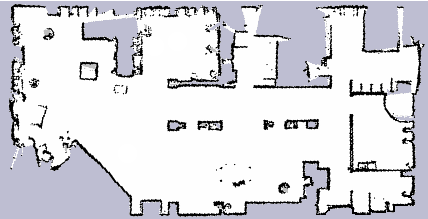
\includegraphics[height=3.25cm]{Figures/Map-2_}};
		\end{tikzpicture}
	\end{center}
	
	\vspace{0.52cm}
	
	\tiny
	
	\textbf{PTracking: Distributed Multi-Agent Multi-Object Tracking through Multi-Clustered Particle
	Filtering} \\
	F. Previtali, L. Iocchi \\
	\emph{IEEE International Conference on Multisensor Fusion and Integration for Intelligent Systems,
	2015} \\
\end{frame}

\begin{frame}
	\frametitle{Quantitative Evaluation}
	\framesubtitle{DIAG}
	
	\small
	
	\begin{table}[!t]
		\centering
		\begin{tabular}{ccccc}
			\cline{1-5}
			\multicolumn{1}{l}{} & \multicolumn{4}{c}{\textbf{\begin{tabular}[c]{@{}c@{}}
			Prey-Predator Distance (avg $ \pm $ std. dev.)\end{tabular}}} \\ \hline
			\multicolumn{1}{c}{\textbf{\#}} & \textbf{Setting 1} & \textbf{Setting 2} &
			\textbf{Setting 3} & \textbf{Setting 4} \\
			
			\multicolumn{1}{c}{1} & 3.04 $ \pm $ 0.63 $ m $ & 2.70 $ \pm $ 0.49
								  $ m $ & 2.02 $ \pm $ 0.38 $ m $ & 1.12 $ \pm $
								  0.19 $ m $ \\
			\multicolumn{1}{c}{2} & 2.95 $ \pm $ 0.80 $ m $ & 2.65 $ \pm $ 0.48
								  $ m $ & 1.95 $ \pm $ 0.42 $ m $ & 1.15 $ \pm $
								  0.20 $ m $ \\
			\multicolumn{1}{c}{3} & 3.12 $ \pm $ 0.53 $ m $ & 2.87 $ \pm $ 0.56
								  $ m $ & 2.03 $ \pm $ 0.41 $ m $ & 1.13 $ \pm $
								  0.19 $ m $ \\
			\multicolumn{1}{c}{4} & 3.01 $ \pm $ 0.69 $ m $ & 2.73 $ \pm $ 0.49
								  $ m $ & 2.06 $ \pm $ 0.38 $ m $ & 1.08 $ \pm $
								  0.22 $ m $ \\
			\multicolumn{1}{c}{5} & 2.99 $ \pm $ 0.72 $ m $ & 2.86 $ \pm $ 0.61
								  $ m $ & 1.99 $ \pm $ 0.40 $ m $ & 1.11 $ \pm $
								  0.17 $ m $ \\
			\hline
			
			\\
			
			\hline
			\multicolumn{1}{l}{} & \multicolumn{4}{c}{\textbf{\begin{tabular}[c]
			{@{}c@{}}Tracking Performance (MOTA,MOTP)\end{tabular}}} \\ \hline
			\multicolumn{1}{c}{\textbf{\#}} & \textbf{Setting 1} & \textbf{Setting 2} &
			\textbf{Setting 3} & \textbf{Setting 4} \\
			
			\multicolumn{1}{c}{1} & (0.63,0.45) & (0.67,0.49) & (0.75,0.51) & (0.94,0.75) \\
			\multicolumn{1}{c}{2} & (0.59,0.42) & (0.65,0.45) & (0.73,0.49) & (0.92,0.74) \\
			\multicolumn{1}{c}{3} & (0.64,0.41) & (0.69,0.48) & (0.70,0.47) & (0.95,0.77) \\
			\multicolumn{1}{c}{4} & (0.62,0.45) & (0.62,0.40) & (0.74,0.50) & (0.92,0.75) \\
			\multicolumn{1}{c}{5} & (0.57,0.39) & (0.64,0.44) & (0.70,0.48) & (0.94,0.77) \\
			\hline
		\end{tabular}
	\end{table}
\end{frame}

\begin{frame}
	\frametitle{Quantitative Evaluation}
	\framesubtitle{Peccioli House}
	
	\small
	
	\begin{table}
		\centering
		\begin{tabular}{ccccc}
			\cline{1-5}
			\multicolumn{1}{l}{} & \multicolumn{4}{c}{\textbf{\begin{tabular}[c]{@{}c@{}}
			Prey-Predator Distance (avg $ \pm $ std. dev.)\end{tabular}}} \\ \hline
			\multicolumn{1}{c}{\textbf{\#}} & \textbf{Setting 1} & \textbf{Setting 2} &
			\textbf{Setting 3} & \textbf{Setting 4} \\
			
			\multicolumn{1}{c}{1} & 2.84 $ \pm $ 0.59 $ m $ & 2.55 $ \pm $ 0.47
								  $ m $ & 1.85 $ \pm $ 0.38 $ m $ & 1.07 $ \pm $
								  0.18 $ m $ \\
			\multicolumn{1}{c}{2} & 2.85 $ \pm $ 0.74 $ m $ & 2.52 $ \pm $ 0.51
								  $ m $ & 1.84 $ \pm $ 0.40 $ m $ & 1.05 $ \pm $
								  0.21 $ m $ \\
			\multicolumn{1}{c}{3} & 3.03 $ \pm $ 0.57 $ m $ & 2.76 $ \pm $ 0.52
								  $ m $ & 1.91 $ \pm $ 0.43 $ m $ & 1.11 $ \pm $
								  0.20 $ m $ \\
			\multicolumn{1}{c}{4} & 3.04 $ \pm $ 0.61 $ m $ & 2.63 $ \pm $ 0.47
								  $ m $ & 1.93 $ \pm $ 0.39 $ m $ & 1.08 $ \pm $
								  0.21 $ m $ \\
			\multicolumn{1}{c}{5} & 2.89 $ \pm $ 0.68 $ m $ & 2.77 $ \pm $ 0.56
								  $ m $ & 1.89 $ \pm $ 0.41 $ m $ & 1.09 $ \pm $
								  0.15 $ m $ \\
			
			\hline
			
			\\
			
			\hline
			\multicolumn{1}{l}{} & \multicolumn{4}{c}{\textbf{\begin{tabular}[c]
			{@{}c@{}}Tracking Performance (MOTA,MOTP)\end{tabular}}} \\ \hline
			\multicolumn{1}{c}{\textbf{\#}} & \textbf{Setting 1} & \textbf{Setting 2} &
			\textbf{Setting 3} & \textbf{Setting 4} \\
			
			\multicolumn{1}{c}{1} & (0.67,0.42) & (0.71,0.49) & (0.78,0.58) & (0.93,0.79) \\
			\multicolumn{1}{c}{2} & (0.62,0.43) & (0.69,0.46) & (0.77,0.55) & (0.95,0.76) \\
			\multicolumn{1}{c}{3} & (0.64,0.47) & (0.73,0.51) & (0.72,0.52) & (0.96,0.79) \\
			\multicolumn{1}{c}{4} & (0.66,0.44) & (0.68,0.43) & (0.75,0.53) & (0.93,0.77) \\
			\multicolumn{1}{c}{5} & (0.60,0.41) & (0.65,0.45) & (0.71,0.51) & (0.97,0.81) \\
			\hline
		\end{tabular}
	\end{table}
\end{frame}

\section{Related Work - Activity Forecasting}

\begin{frame}
	\frametitle{Related Work}
	\framesubtitle{Human Activity Classification and Activity Recognition}
	
	\vspace{0.4cm}
	
	\begin{columns}[T]
		\column{.55\textwidth}
		
		\vspace{0.2cm}
		
		\begin{itemize}
			\item \textbf{Nascimento {et al.} \cite{Nascimento10}:} recognise pedestrian trajectories in
				  video sequences, in a surveillance context
			
			\vspace{1.2cm}
			
			\item \textbf{Veloso {et al.} \cite{Vail07}:} discriminatively trained Conditional Random
				  Fields for activity recognition
		\end{itemize}
		
		\column{.5\textwidth}
		
		\centering
		\begin{tikzpicture}
			\node at (1.42,0) [draw=black,ultra thick,inner sep=0pt]
			{
				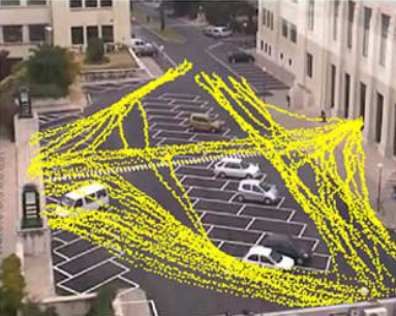
\includegraphics[height=2.2cm]{Figures/Nascimento-1}
			};
			\node at (-1.42,0) [draw=black,ultra thick,inner sep=0pt]
			{
				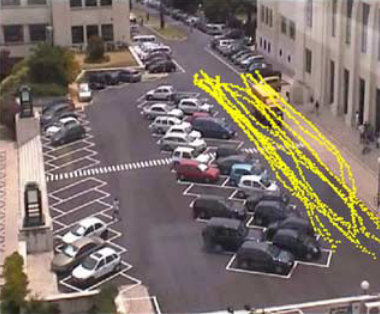
\includegraphics[height=2.2cm]{Figures/Nascimento-2}
			};
			\node at (0,-2.8) [draw=black,ultra thick,inner sep=0pt]
			{
				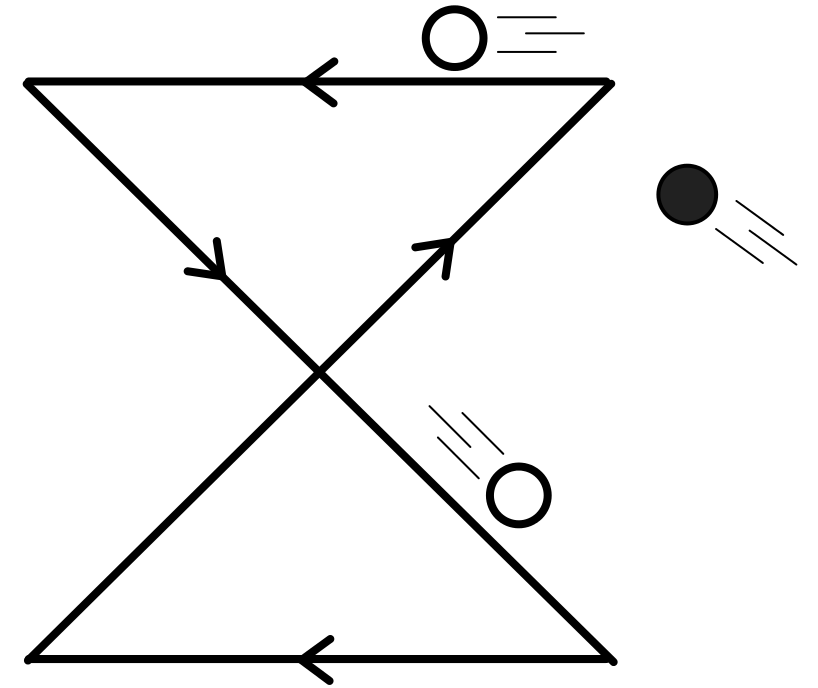
\includegraphics[width=3.6cm]{Figures/Veloso}
			};
		\end{tikzpicture}
	\end{columns}
	
	\vspace{0.47cm}
	
	\tiny
	
	\cite{Nascimento10} J. C. Nascimento \emph{et al.}, ``Trajectory classification using switched
	dynamical hidden Markov models'', Image Processing, 2010
	
	\vspace{-0.17cm}
	
	\cite{Vail07} D. L. Vail \emph{et al.}, ``Conditional random fields for activity recognition'',
	AAMAS, 2007
\end{frame}

\begin{frame}
	\frametitle{Related Work}
	\framesubtitle{Activity Forecasting through Semantic Mapping}
	
	\vspace{0.33cm}
	
	\large
	
	\textbf{Ziebart \emph{et al.} \cite{Kitani12}} propose a method for activity forecasting by
	combining:
	
	\begin{itemize}
		\item Semantic scene understanding
		\vspace{0.05cm}
		\item Inverse Optimal Control
	\end{itemize}
	
	\vspace{-0.2cm}
	
	\begin{center}
		\begin{tikzpicture}
			\node at (0,0) [draw=white,ultra thick,inner sep=0pt]
			{
				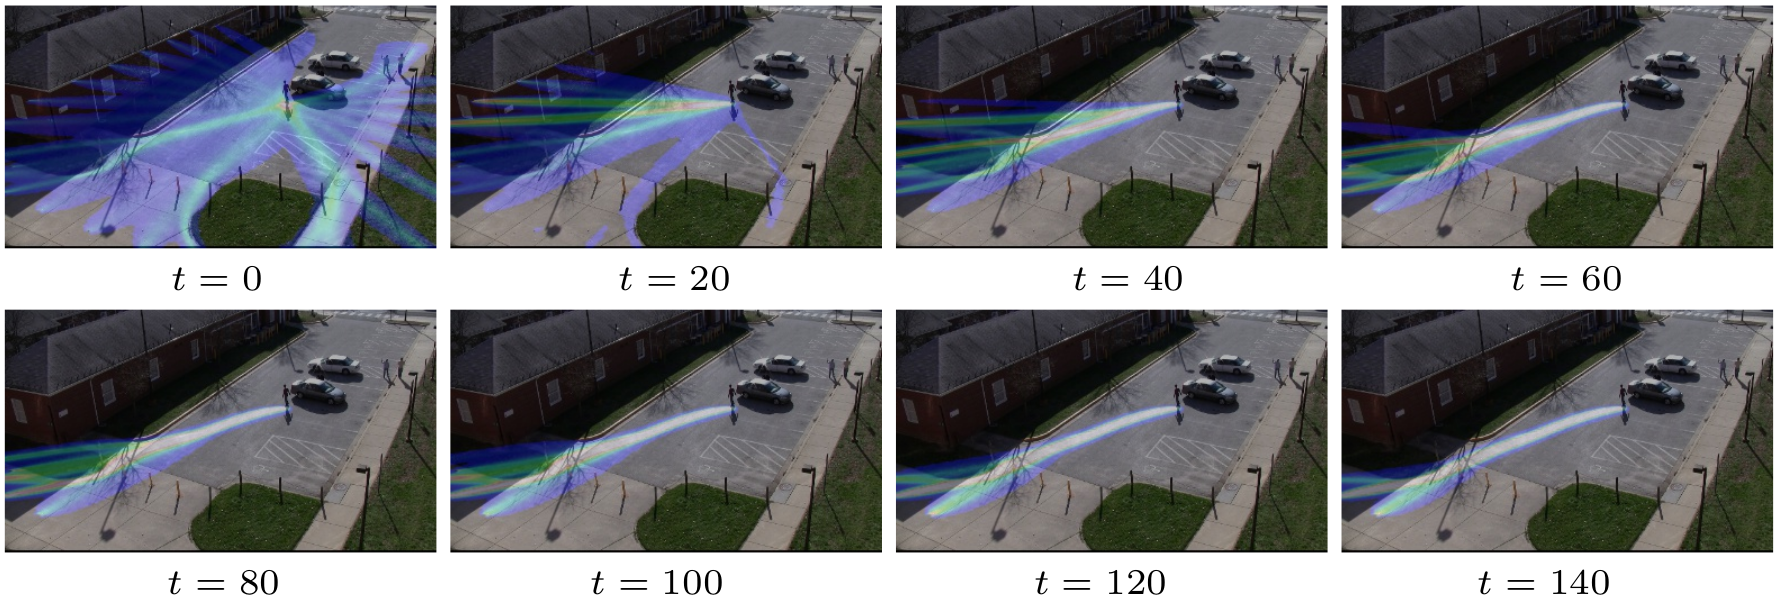
\includegraphics[scale=0.19]{Figures/ActivityForecasting.png}
			};
		\end{tikzpicture}
	\end{center}
	
	\vspace{-0.3cm}
	
	\tiny
	
	\cite{Kitani12} K. Kitani \emph{et al.}, ``Activity Forecasting'', ECCV, 2012
\end{frame}

\begin{frame}
	\frametitle{Advantages/Disadvantages}
	
	\Large
	
	\vspace{0.4cm}
	
	\underline{\textbf{Advantages}} \\
	
	\vspace{0.2cm}
	
	\begin{itemize}
		\item Knowledge transfer by using physical scene features
		\item Accurate and robust destination forecasting
	\end{itemize}
	
	\vspace{0.2cm}
	
	\underline{\textbf{Disadvantages}} \\
	
	\vspace{0.19cm}
	
	\begin{itemize}
		\item Prior knowledge of potential goals
		\item Space of possible motions is explicitly parametrised
		\item Applicability in dynamic environments? \\
			  \vspace{-0.2cm}
			  \begin{tabbing}
				  \hspace{0.3cm}
				  \large
				  $ \leadsto $ \emph{rescue or rapidly changing construction environment}
			  \end{tabbing}
	\end{itemize}
\end{frame}

\section{Activity Forecasting}

\logo
{
	\begin{tikzpicture}
		\hspace{0.09cm}
		\node at (-1,0) [draw=white,ultra thick,inner sep=0pt]
		{
			\includegraphics[height=1cm]{ThemeFigs/Sapienza}
		};
		\node at (0,0) [draw=white,ultra thick,inner sep=0pt]
		{
			\includegraphics[height=1cm]{ThemeFigs/Edinburgh}
		};
	\end{tikzpicture}
	\vspace{199.1pt}
}

\begin{frame}
	\frametitle{Predicting Future Agent Motions}
	
	\vspace{0.2cm}
	
	\begin{block}{Idea}
		Performing activity forecasting resolving an \textbf{Inverse Reinforcement Learning} problem
		\textbf{without} needing a labelled environment, by combining:
		\vspace{0.05cm}
		\begin{itemize}
			\item Object trajectories provided by \emph{PTracking}
			\item Representation of the environment following the \emph{grid world} schema defined by
				  Russell et al. \cite{Ng00}
		\end{itemize}
	\end{block}
	
	\vspace{-0.1cm}
	
	\begin{center}
		\begin{tikzpicture}
			\node at (0,0) [draw=white,ultra thick,inner sep=0pt]
			{
				\includegraphics[height=3.2cm]{Figures/IRL}
			};
		\end{tikzpicture}
	\end{center}
	
	\vspace{-0.34cm}
	
	\tiny
	
	\cite{Ng00} A. Y. Ng \emph{et al.},  ``Algorithms for inverse reinforcement learning'', ICML, 2000
\end{frame}

%\begin{frame}
%	\frametitle{Predicting Future Agent Motions}
%	\framesubtitle{Contributions}
%	
%	\Large
%	
%	\vspace{0.4cm}
%	
%	We propose an integrated framework, which relies on \emph{PTracking}, for estimating future movement
%	intentions of goal-oriented agents, that:
%	
%	\vspace{0.15cm}
%	
%	\begin{enumerate}
%		\item \textbf{Does not} rely on semantic scene labelling
%		\item \textbf{Incrementally} updates the IRL model over time
%		\item Makes use of \textbf{non-uniform grids} for representing the state of the environment
%	\end{enumerate}
%\end{frame}

\begin{frame}
	\frametitle{Predicting Future Agent Motions}
	\framesubtitle{Approach}
	
	\vspace{-0.1cm}
	
	\begin{columns}[T]
		\column{.4\textwidth}
		
		\vspace{-0.2cm}
		
		\begin{equation*}
			\hspace{0.3cm}
			\scriptsize
			\begin{array}{ll}
				\min \sum\nolimits_{i=1}^N -x_i + \lambda (r_i^+ - r_i^-)
				\vspace{-0.35cm} \\ \\
				s.t. \\ \;\;\;\;
				\left \{
					\begin{array}{ll}
						x_i \leq (\mathbf{P}_{a_*} - \mathbf{P}_a)(\mathbf{I} - \gamma
						\mathbf{P}_{a_*})^{-1} \mathbf{R} \\
						\vspace{-0.25cm} \\
						\;\;\;\;\;\;\;\;\;\;\;\;\;\;\;\;\;\;\;\;\;
						\;\;\; \forall \, a \in \mathbf{A}, \; i \in \{ 1, \ldots, N \}
						\vspace{-0.25cm}\\ \\
						x_i \geq 0 \;\;\;\;\;\;\,\,\,\,\;\;\;\,\,\,\,\,\;\,\,\,\,\,\,\,\;\;\;\;\;
						\;\,\,\,\,\, i \in \{ 1, \ldots, N \}
						\vspace{-0.25cm} \\ \\
						r_i = r_i^+ + r_i^- \;\,\,\,\,\,\;\,\,\,\,\,\,\,\;\;\;\;\;
						\;\,\,\,\,\, i \in \{ 1, \ldots, N \}
						\vspace{-0.25cm}
						\\ \\
						| \mathbf{R}_i | \leq R_{max} \;\;\;\;\;\;\;\;\;\;\;\,\,\,\,\;\;\
						\,\,\,\,\,\, i \in \{ 1, \ldots, N \}
					\end{array}
				\right.
				\vspace{0.2cm}
			\end{array}
		\end{equation*}
		
		\tiny
		
		\vspace{-0.8cm}
		
		\begin{tabbing}
			\hspace{0.2cm}
			Adapted formalisation of [Ng \& Russel, 2000]
		\end{tabbing}
		
		\vspace{-1cm}
		
		\column{.15\textwidth}
		
		\centering
		\vspace{1.3cm}
		
		\begin{tabbing}
			\hspace{1.5cm}
			\Huge
			\textcolor{red}{\textbf{+}}
		\end{tabbing}
		
		\column{.45\textwidth}
		\centering
		
		\vspace{0.4cm}
		
		\begin{tikzpicture}
			\node at (0,0) [draw=black,ultra thick,inner sep=0pt]
			{
				\includegraphics[width=4.8cm]{Figures/RecursiveNonUniformGrids}
			};
		\end{tikzpicture}
	\end{columns}
	
	\vspace{0.2cm}
	
	\begin{columns}[T]
		\column{.35\textwidth}
		
		\begin{tikzpicture}
			\hspace{0.2cm}
			\centering
			\node at (0,0) [draw=white,ultra thick,inner sep=0pt]
			{
				\includegraphics[height=3.2cm]{Figures/IRL-Model}
			};
		\end{tikzpicture}
		
		\column{.2\textwidth}
		
		\centering
		\vspace{1.1cm}
		
		\begin{tabbing}
			\hspace{1.975cm}
			\Huge
			\textcolor{red}{\textbf{$ \Rightarrow $}}
		\end{tabbing}
		
		\column{.45\textwidth}
		\centering
		
		\begin{tikzpicture}
			\node at (0,0) [draw=black,ultra thick,inner sep=0pt]
			{
				\includegraphics[width=4.8cm]{Figures/Motivation}
			};
		\end{tikzpicture}
	\end{columns}
	
	\begin{columns}[T]
		\column{\textwidth}
		
		\centering
		\vspace{-3.1cm}
		\hspace{-1cm}
		\Huge
		\begin{rotate}{-45}
			
			\textcolor{blue}{\textbf{$ \Downarrow $}}
		\end{rotate}	
	\end{columns}
\end{frame}

\begin{frame}
	\frametitle{Predicting Future Agent Motions}
	\framesubtitle{Policy Generation}
	
	\vspace{0.2cm}
	
	\begin{center}
		\begin{tikzpicture}
			\node at (-4.3,-1) [draw=black,ultra thick,inner sep=0pt]
			{
				\includegraphics[width=0.5\linewidth]{Figures/Reward-3}
			};
			\node at (1,1) [draw=black,ultra thick,inner sep=0pt]
			{
				\includegraphics[width=0.45\linewidth]{Figures/Reward-2}
			};
			\node at (-4,1.7) [draw=black,ultra thick,inner sep=0pt]
			{
				\includegraphics[width=0.5\linewidth]{Figures/Reward-1}
			};
		\end{tikzpicture}
	\end{center}
	
	Goals can be \emph{statically} chosen or \emph{generated} by analysing tracking data
\end{frame}

%\begin{frame}
%	\frametitle{Predicting Future Agent Motions}
%	\framesubtitle{Observed Trajectory Extraction}
%	
%	\LARGE
%	
%	\vspace{0.4cm}
%	
%	We gather object estimates from \emph{PTracking} considering an arbitrary temporal window. \\
%	
%	\vspace{0.4cm}
%	
%	Having acquired a set of trajectories $ \mathcal{U} $, we \textbf{ground} each trajectory $ u \in
%	\mathcal{U} $ in every policy $ \pi_s^G $. \\
%\end{frame}

\begin{frame}
	\frametitle{Predicting Future Agent Motions}
	\framesubtitle{Policy Comparison}
	
	\Large
	
	\vspace{0.3cm}
	
	Best fitting policy by \textbf{comparing} the target trajectory against trajectories drawn from
	potential optimal policies.
	
	\vspace{-0.3cm}
	
	\begin{center}
		\begin{tikzpicture}
			\node at (0,0) [draw=white,ultra thick,inner sep=0pt]
			{
				\includegraphics[width=0.72\linewidth]{Figures/Frechet}
			};
		\end{tikzpicture}
	\end{center}
	
	\vspace{-0.5cm}
	
	The \textbf{Fr\'echet distance} between curves is the minimum leash length that permits the walk.\\
\end{frame}

\begin{frame}
	\frametitle{Predicting Future Agent Motions}
	\framesubtitle{Goal Prediction}
	
	\Large
	
	\vspace{0.25cm}
	
	We \textbf{predict in real-time} the goal toward which each moving object is likely to be headed,
	by executing the policy that best matches its movement pattern.
	
	\vspace{-0.1cm}
	
	\begin{center}
		\begin{tikzpicture}
			\node at (0,0) [draw=black,ultra thick,inner sep=0pt]
			{
				\includegraphics[width=0.59\linewidth]{Figures/Motivation}
			};
		\end{tikzpicture}
	\end{center}
\end{frame}

%\begin{frame}
%	\frametitle{Predicting Future Agent Motions}
%	\framesubtitle{Anomaly Detection}
%	
%	\LARGE
%	
%	\vspace{0.5cm}
%	
%	It could happen that a trajectory $ u \in \mathcal{U} $ does not match any model:
%	\begin{itemize}
%		\item A trajectory fragment $ u $ is \textbf{anomalous} and refers to a \emph{suspicious
%			  activity pattern}
%		\item Environment has changed leading to new types of motion
%			  \vspace{-0.25cm}
%			  \begin{tabbing}
%				  \hspace{0.3cm}
%				  \large
%				  $ \leadsto $ \emph{can be recognised by analysing the foreground model}
%			  \end{tabbing}
%	\end{itemize}
%\end{frame}

\section{Experimental Evaluation - Activity Forecasting}

\begin{frame}
	\frametitle{}
	
	\Huge
	
	\vspace{0.5cm}
	
	\begin{center}
		\textbf{Experimental Evaluation\\ Activity Forecasting}
	\end{center}
\end{frame}

\begin{frame}
	\frametitle{Evaluating an Activity Forecasting Algorithm}
	
	\Large
	
	\vspace{0.45cm}
	
	The Negative Log-Loss (NLL) represents the expectation of the log-likelihood of a trajectory $ s $
	under a policy $ \pi(a \, | \, s) $:
	\vspace{-0.1cm}
	\begin{equation*}
		NLL(s) = E_{\pi(a \, | \, s)} \Big [ -\log \prod\nolimits_t \pi(a_t \, | \, s_t)  \Big ]
	\end{equation*}
	
	\vspace{0.1cm}
	
	This metric measures the probability of drawing the demonstrated trajectory from the learnt
	distribution over all possible trajectories. \\
\end{frame}

\begin{frame}
	\frametitle{Experimental Evaluation}
	\framesubtitle{Activity Forecasting}
	
	\large
	
	\vspace{-0.1cm}
	
	\begin{columns}[t]
		\only<1->
		{
			\column{0.9\textwidth}
			
			\begin{block}{Predicting Future Agent Motions}
				inferring agent goals accurately in a varied set of environments
			\end{block}
			
			\column{0.05\textwidth}
		}
	\end{columns}
	
	\vspace{0.1cm}
	
	\begin{center}
		\begin{tikzpicture}
			\node at (0,0) [draw=black,ultra thick,inner sep=0pt]  {\includegraphics[height=2.9cm]{Figures/InformaticsForum}};
			\node at (4,0) [draw=black,ultra thick,inner sep=0pt]  {\includegraphics[height=2.9cm]{Figures/InSpace_FrontCamera}};
			\node at (7.98,0) [draw=black,ultra thick,inner sep=0pt]  {\includegraphics[height=2.9cm]{Figures/VIRAT}};
		\end{tikzpicture}
	\end{center}
	
	\vspace{0.15cm}
	
	\tiny
	
	\textbf{IRL-based Prediction of Goals for Dynamic Environments}\\
	F. Previtali, A. Bordallo, S. Ramamoorthy \\
	\emph{Workshop on Machine Learning for Social Robotics at ICRA, 2015} \\
	
	\vspace{0.1cm}
	
	\textbf{Predicting Future Agent Motions for Dynamic Environments}\\
	F. Previtali, A. Bordallo, L. Iocchi, S. Ramamoorthy \\
	\emph{International Conference on Intelligent Robots and Systems} [submitted] \\
\end{frame}

\begin{frame}
	\frametitle{Quantitative Evaluation}
	\framesubtitle{Activity Forecasting}
	
	\begin{figure}
		\centering
		\begin{tikzpicture}
			\node at (0,0) [draw=white,ultra thick,inner sep=0pt]
			{
				\includegraphics[width=\linewidth]{Figures/QuantitativeEvaluation}
			};
		\end{tikzpicture}
	\end{figure}
\end{frame}

\begin{frame}
	\frametitle{Qualitative Evaluation}
	\framesubtitle{InSpace}
	
	\begin{figure}[!h]
		\centering
		\includemovie[inline=false,text=
		{
			\begin{tikzpicture}
				\node at (0,0) [draw=black,ultra thick,inner sep=0pt]
				{
					\includegraphics[width=0.65\linewidth]{Figures/InSpace_FrontCamera}
				};
			\end{tikzpicture}
		}]{}{}{../Videos/5-ActivityForecasting/PTracking-House.avi}
	\end{figure}
\end{frame}

\begin{frame}
	\frametitle{Experimental Evaluation}
	\framesubtitle{Context-Aware Navigation}
	
	\large
	
	\begin{columns}[t]
		\only<1->
		{
			\column{0.84\textwidth}
			
			\begin{block}{Inferring Target Goals}
				intention-inference for dynamic environments with multiple interactively navigating
				agents
			\end{block}
			
			\column{0.11\textwidth}
		}
	\end{columns}
	
	\vspace{0.2cm}
	
	\begin{center}
		\begin{tikzpicture}
			\node at (0,0) [draw=black,ultra thick,inner sep=0pt]  {\includegraphics[height=2.9cm]{Figures/Kinect-1}};
			\node at (4,0) [draw=black,ultra thick,inner sep=0pt]  {\includegraphics[height=2.9cm]{Figures/Kinect-2}};
			\node at (8,0) [draw=black,ultra thick,inner sep=0pt]  {\includegraphics[height=2.9cm]{Figures/Kinect-3}};
		\end{tikzpicture}
	\end{center}
	
	\vspace{0.3cm}
	
	\tiny
	
	\textbf{Counterfactual Reasoning about Intent for Interactive Navigation in Dynamic Environments}\\
	A. Bordallo, F. Previtali, N. Nardelli, S. Ramamoorthy \\
	\emph{IEEE/RSJ International Conference on Intelligent Robots and Systems, 2015} \\
\end{frame}

\begin{frame}
	\frametitle{Qualitative Evaluation}
	\framesubtitle{InSpace}
	
	\begin{figure}[!h]
		\centering
		\includemovie[inline=false,text=
		{
			\begin{tikzpicture}
				\node at (0,0) [draw=black,ultra thick,inner sep=0pt]
				{
					\includegraphics[width=0.65\linewidth]{Figures/InSpace}
				};
			\end{tikzpicture}
		}]{}{}{../Videos/3-Youbot/PTracking-2People_3PlanningYoubots.mpg}
	\end{figure}
\end{frame}

\begin{frame}
	\frametitle{Experimental Evaluation}
	\framesubtitle{Interactive Costmaps}
	
	\large
	
	\begin{columns}[t]
		\only<1->
		{
			\column{0.8\textwidth}
			
			\begin{block}{Effective Social Motion Planning}
				reasoning about interactive agents' intention in the environment in order to adapt the
				costmap over time
			\end{block}
			
			\column{0.15\textwidth}
		}
	\end{columns}
	
	\vspace{0.2cm}
	
	\begin{center}
		\begin{tikzpicture}
			\node at (0,0) [draw=black,ultra thick,inner sep=0pt]  {\includegraphics[height=2.8cm]{Figures/ConstantVelocityComparison}};
			\node at (4.05,0) [draw=black,ultra thick,inner sep=0pt]  {\includegraphics[height=2.8cm]{Figures/ProxemicsComparison}};
			\node at (8.11,0) [draw=black,ultra thick,inner sep=0pt]  {\includegraphics[height=2.8cm]{Figures/InteractiveCostmapComparison}};
		\end{tikzpicture}
	\end{center}
	
	\vspace{0.36cm}
	
	\tiny
	
	\textbf{Interactive Costmaps: Integrating Prediction and Planning with Counterfactual Reasoning}\\
	A. Bordallo, F. Previtali, S. Ramamoorthy \\
	\emph{IEEE/RSJ International Conference on Intelligent Robots and Systems, 2015} [submitted] \\
\end{frame}

\begin{frame}
	\frametitle{Quantitative Evaluation}
	\framesubtitle{InSpace}
	
	\begin{table}
	\centering
	\caption{Comparison of costmap experiments, obstacle layer is used as a baseline. CPU\% shows
			 average measured consumption and p.a. shows additional load per agent. Execution time shows
			 time required for costmap generation. Experiment times show average/worst time over all
			 trials, where $\infty s$ denotes a timeout.}
	\def\arraystretch{1.3}
	\vspace{-0.3cm}
	\resizebox{\textwidth}{!}
	{
		\begin{tabular}{lcccccc}
Method & CPU & Execution Time & Passing Time & Crossing Time & Collisions & Near-collision \\ 
\hline
Obstacle layer (Baseline) & -\% & -s & 5/$\infty$s & 5/$\infty$s & 80\% & 70\%  \\
Constant Velocity model & 4\%+1\% p.a. & 5ms p.a. & 15/20s & 12/18s & 40\% & 60\%  \\
Proxemics and social & 3\%+2\% p.a. & 5ms + 5ms p.a. & 8/28s & 12/14s & 20\% &  50\%  \\
\textbf{Interactive Costmap} & \textbf{6\%+2\% p.a.} & \textbf{5ms + 5ms p.a.} & \textbf{7/8s} & \textbf{8/9s} & \textbf{10\%} &  \textbf{20\%}  \\
		\end{tabular}
	}
\end{table}
\end{frame}

\begin{frame}
	\frametitle{Qualitative Evaluation}
	\framesubtitle{InSpace}
	
	\begin{figure}[!h]
		\centering
		\includemovie[inline=false,text=
		{
			\begin{tikzpicture}
				\node at (0,0) [draw=black,ultra thick,inner sep=0pt]
				{
					\includegraphics[width=0.65\linewidth]{Figures/InteractiveCostmap}
				};
			\end{tikzpicture}
		}]{}{}{../Videos/3-Youbot/InteractiveCostmaps.avi}
	\end{figure}
\end{frame}

\section{Conclusions}

\begin{frame}
	\frametitle{Conclusions}
	
	\Large
	
	\vspace{0.3cm}
	
	We presented:
	
	\begin{enumerate}
		\item \emph{PTracking}, a novel \textbf{real-time} distributed tracker
		\item \textbf{Effective} framework for \textbf{predicting} future agent motions of
			  goal-oriented agents
	\end{enumerate}
	
	\vspace{0.2cm}
	
	\underline{\textbf{Main contributions}}
	
	\begin{itemize}
		\item Real-time, accurate and precise tracking
		\item Fully scalable design
		\item Prediction without prior annotation of scene semantics
		\item Non-uniform grids for state representation
		\item Efficient and scalable for on-robot implementation
	\end{itemize}
\end{frame}

\begin{frame}
	\frametitle{Future Work}
	
	\Large
	
	Possible future directions in terms of tracking could be:
	\begin{itemize}
		\item \textbf{Integration} of recent real-time \textbf{feature extractors} in the data
			  association module
		\item \textbf{Generation} of a \textbf{3D model} by merging information coming from multiple
			  sources
	\end{itemize}
	
	while, in terms of prediction of future agent motions could be the employment of \textbf{more
	sophisticated} \emph{IRL} alternatives within the overall proposed framework.\\
\end{frame}

\logo{}

\begin{frame}
	\frametitle{Major Reviewers' Comments}
	
	\large
	
	\textbf{Rev.}\\
	``For some experiments, comparisons are only made with various versions of the same algorithms.''
	
	\vspace{0.3cm}
	
	\textbf{Rev.}\\
	``The benefits of the method are shown for activity forecasting applications, intention prediction,
	and for constructing interactive costmaps to guide robot navigation. The latter applications
	represent significant contributions in robotics. Some additional discussion of the assumptions being  
	employed would be useful. Specifically, the joint optimization seems to assume more coordination
	than, e.g., humans have when they navigate (often sub-­optimally).'' \\
\end{frame}

\logo
{
	\begin{tikzpicture}
		\hspace{0.09cm}
		\node at (-1,0) [draw=white,ultra thick,inner sep=0pt]
		{
			\includegraphics[height=1cm]{ThemeFigs/Sapienza}
		};
		\node at (0,0) [draw=white,ultra thick,inner sep=0pt]
		{
			\includegraphics[height=1cm]{ThemeFigs/Edinburgh}
		};
	\end{tikzpicture}
	\vspace{199.1pt}
}

\begin{frame}
	\frametitle{Full List of Publications}
	
	\vspace{-0.2cm}
	
	\begin{columns}[t]
		\column{0.48\textwidth}
		
		\tiny
		
		\textcolor{red}{\textbf{\underline{Journal}}}
		
		\vspace{0.1cm}
		
		\textbf{1. Multi-Robot Surveillance through a Distributed Sensor Network}, A. Pennisi, F.
		Previtali, C. Gennari, D. D. Bloisi, L. Iocchi, F. Ficarola, A. Vitaletti, D. Nardi \\
		\emph{Journal of Studies in Computational Intelligence, 2015}
		
		\vspace{0.15cm}
		
		\textbf{2. Distributed Sensor Network for Multi-Robot Surveillance}, A. Pennisi, F. Previtali,
		F. Ficarola, D. D. Bloisi, L. Iocchi, A. Vitaletti \\
		\emph{Procedia Computer Science, 2014}
		
		\vspace{0.2cm}
		
		\textcolor{red}{\textbf{\underline{Conference}}}
		
		\vspace{0.1cm}
		
		\textbf{3. PTracking: Distributed Multi-Agent Multi-Object Tracking through Multi-Clustered
		Particle Filtering}, F. Previtali, L. Iocchi \\
		\emph{IEEE Conference on Multisensor Fusion and Integration, 2015}
		
		\vspace{0.15cm}
		
		\textbf{4. Disambiguating Localization Symmetry through a Multi-Clustered Particle Filtering},
		F. Previtali, G. Gemignani, L. Iocchi, D. Nardi \\
		\emph{IEEE Conference on Multisensor Fusion and Integration, 2015}
		
		\vspace{0.15cm}
		
		\textbf{5. Counterfactual Reasoning about Intent for Interactive Navigation in Dynamic
		Environments}, A. Bordallo, F. Previtali, N. Nardelli, S. Ramamoorthy \\
		\emph{IEEE Conference on Intelligent Robots and Systems, 2015}
		
		\vspace{0.15cm}
		
		\textbf{6. IRL-based Prediction of Goals for Dynamic Environments}, F. Previtali, A. Bordallo,
		S. Ramamoorthy \\
		\emph{Machine Learning for Social Robotics at ICRA, 2015}
		
		\column{0.53\textwidth}
		
		\vspace{0.34cm}
		
		\tiny
		
		\textbf{7. Real-Time Adaptive Background Modeling in Fast Changing Conditions}, A. Pennisi, F.
		Previtali, D. D. Bloisi, L. Iocchi \\
		\emph{Conference on Advanced Video and Signal based Surveillance, 2015}
		
		\vspace{0.2cm}
		
		\textcolor{red}{\textbf{\underline{Submitted}}}
		
		\vspace{0.1cm}
		
		\textbf{8. A Distributed Approach for Real-Time Multi-Camera Multi-Object Tracking}, F.
		Previtali, D. D. Bloisi, L. Iocchi \\
		\emph{Journal on Machine Vision and Applications}
		
		\vspace{0.15cm}
		
		\textbf{9. Enhancing Automatic Maritime Surveillance Systems with Visual Information}, D. D.
		Bloisi, F. Previtali, A. Pennisi, D. Nardi, M. Fiorini \\
		\emph{Transaction on Intelligent Transportation Systems}
		
		\vspace{0.15cm}
		
		\textbf{10. Predicting Future Agent Motions for Dynamic Environments}, F. Previtali, A.
		Bordallo, L. Iocchi, S. Ramamoorthy \\
		\emph{IEEE Conference on Intelligent Robots and Systems}
		
		\vspace{0.15cm}
		
		\textbf{11. Interactive Costmaps: Integrating Prediction and Planning with Counterfactual
		Reasoning}, A. Bordallo, F. Previtali, S. Ramamoorthy \\
		\emph{IEEE Conference on Intelligent Robots and Systems}
	\end{columns}
\end{frame}

\logo{}

\begin{frame}
	\frametitle{That's all!}
	
	\begin{figure}
		\centering
		\begin{tikzpicture}
			\node at (0,0) [draw=white,ultra thick,inner sep=0pt]
			{
				\includegraphics[width=0.8\linewidth]{Figures/Question}
			};
		\end{tikzpicture}
	\end{figure}
\end{frame}


\tiny
\bibliographystyle{plain}
\bibliography{Main}

\end{document}
